\documentclass[a4paper,12pt,twoside]{book}
\usepackage[T1]{fontenc}
\usepackage{inputenc}
\usepackage{fontspec}
\usepackage{lmodern}
\usepackage{xcolor} % colors
\usepackage[english,french]{babel}
\usepackage{xspace} % pour la gestion des espaces après les commandes
%\usepackage{minted} % colored source code
\usepackage{csquotes}
\usepackage{float}

% Mise en page École des chartes
\usepackage[margin=2.5cm]{geometry} % marges
\usepackage{setspace}
\onehalfspacing % interligne de 1.5
\setlength\parindent{1cm}

\usepackage{tocbibind}
\usepackage[backend=biber, sorting=nyt, style=enc, minbibnames=10, maxbibnames=10]{biblatex}
\addbibresource{bibliographie/biblio_astro.bib}
\addbibresource{bibliographie/biblio_computervision.bib}
\nocite{*}
\defbibnote{intro}{Cette bibliographie présente toutes les ressources utilisées, de tout type, citées ou non, par simple ordre alphabétique.}

\usepackage[pdfusetitle, pdfsubject={Mémoire TNAH — Titre}, pdfkeywords={mot1, mot2, mot3}]{hyperref}

\usepackage{graphicx}
\usepackage{subcaption}

\author{Prénom Nom – M2 TNAH — ENC}
\title{Titre mémoire}

% ACRONYMS
\usepackage[automake, acronym, toc]{glossaries}
\makeglossaries
\setacronymstyle{short-long}
\newacronym{fair}{\textsc{fair}}{\emph{Findable Accessible Interoperable Reusable}}
\newacronym{api}{\textsc{api}}{\emph{Application Programming Interface}}
\newacronym{eida}{EIDA}{Editing and analysing hIstorical astronomical Diagrams with Artificial intelligence}
\newacronym{htr}{HTR}{Handwritten Text Recognition}
\newacronym{ocr}{OCR}{Optical Character Recognition}
\newacronym{enherit}{EnHerit}{Enhancing Heritage Image Databases}
\newacronym{vhs}{VHS}{Computer vision and Historical analysis of Scientific illustration circulation}
\newacronym{lte}{LTE}{Laboratoire Temps Espace}
\newacronym{dishas}{DISHAS}{Digital Information System for the History of Astral Science}
\newacronym{bnf}{BNF}{Bibliothèque Nationale de France}
\newacronym{iiif}{IIIF}{International Image Interoperability Framework}
\newacronym{gpu}{GPU}{Graphics Processing Unit}
\newacronym{sql}{SQL}{Structured Query Language}

% COMMANDS
\newcommand{\enc}{École nationale des chartes\xspace}
\newcommand{\fair}{\gls{fair}\xspace}
\newcommand{\api}{\gls{api}\xspace}
\newcommand{\XIV}{\textsc{xiv}\ieme{}\xspace}
% Pour retirer le titre courant d'une page vide avant un chapitre
\newcommand{\clearemptydoublepage}{\newpage{\pagestyle{empty}\cleardoublepage}}
% Pour des sections non numérotées dans la table des matière
\newcommand\chapterNo[1]{
	\chapter*{#1}
	\markright{\MakeUppercase{#1}}
}

% Corrections Som
\newcommand{\som}[1]{\textcolor{teal}{SOM: #1}}

\begin{document}
	
	\onehalfspacing 
	
	\frontmatter
	
	\begin{titlepage}
	\begin{center}
		
		\bigskip
		
		\begin{large}
			ÉCOLE NATIONALE DES CHARTES
		\end{large}
		\begin{center}\rule{2cm}{0.02cm}\end{center}
		
		\bigskip
		\bigskip
		\bigskip
		\begin{Large}
			\textbf{Lucie Ledieu}\\
		\end{Large}
		\begin{normalsize} \textit{licencié ès lettres}\\
		\end{normalsize}
		
		\bigskip
		\bigskip
		\bigskip
		
		\begin{Huge}
			\textbf{Explorer les réseaux de transmission de données historiques}\\
		\end{Huge}
		\bigskip
		\bigskip
		\begin{LARGE}
			\textbf{Élaboration de visualisations pour l'application AIKON}\\
		\end{LARGE}
		
		\bigskip
		\bigskip
		\bigskip
		\begin{large}
		\end{large}
		\vfill
		
		\begin{large}
			Mémoire pour le diplôme de master \\
			\og Technologies numériques appliquées à l'histoire~\fg\\
			\bigskip
			2025
		\end{large}
		
	\end{center}
\end{titlepage}
	
	\thispagestyle{empty}	
	\cleardoublepage
	
	\chapterNo{Résumé}
\addcontentsline{toc}{chapter}{Résumé}
\medskip	

Résumé\\

\textbf{Mots-clés~:} mot1~; mot2~; mot3~.\\

\textbf{Informations bibliographiques~:} Prénom Nom, \textit{Titre du mémoire}, mémoire de master \og Technologies numériques appliquées à l'histoire~\fg, dir. Prénom Nom, École nationale des chartes, 20**.

\clearemptydoublepage
	
	\chapterNo{Remerciements}
	\addcontentsline{toc}{chapter}{Remerciements}
	
	\chapterNo{Introduction}
	\addcontentsline{toc}{chapter}{Introduction}
	
	La mission principale de ce stage était de concevoir des preuves de concept pour des visualisations à partir des données des projets EIDA et VHS. Ces dernières ont pour but de tester la faisabilité et la pertinence de visualisations à intégrer au sein de l’application de traitement semi-automatique de données AIKON. Avant de les développer, j’ai rédigé un cahier des charges et un benchmark des solutions techniques envisageables. Ces livrables techniques m’ont permis de définir des objectifs clairs ainsi que les limites de mon projet. Afin de bien comprendre le fonctionnement de l’application AIKON et l’expérience utilisateur qu’elle procure, j’ai rédigé une documentation pour les différentes fonctionnalités de l’interface utilisateur. Pour clore ce stage, un Digital Humanities Seminar a été organisé pour partager aux chercheurs mes recherches, les différentes étapes de réalisation des visualisations et les résultats obtenus. Plus largement, ce travail m’a amené à réaliser une réflexion approfondie autour du concept de visualisation des données en sciences humaines et sociales que je vais exposer dans ce mémoire. 
	
	
	\thispagestyle{empty}
	\cleardoublepage
	
	\mainmatter
	
	\part{Enjeux scientifiques et techniques de l'analyse automatisée des transmissions iconographiques}

	
	\chapter[Les diagrammes astronomiques]{Les diagrammes astronomiques comme objets d'étude des circulations visuelles}
	
		\som{Attention à l'effet "liste" avec trois points de suspension à la fin, essayer de contextualiser l'existence des images en parallèle du texte (outil d'étude central de l'histoire) : c'est le fait de travailler sur des images plutôt que du texte qui donne son intérêt à la méthodologie d'EIDA donc donner un cadre serait intéressant. De même, accentuer dans le second paragraphe la notion de circulation, de copie, et la spécificité de la circulation des images par rapport au texte (pas conditionnées par une langue par ex). Faire intervenir EIDA comme un exemple de cette étude visuelle : retrace en effet la trajectoire des idées, mais s'intéresse surtout à la circulation des diagrammes à travers des traditions diverses, sans limitation de langue, dans un vaste cadre chrono/géo.}
	
	L'histoire des sciences nous offre une grande diversité de représentations iconographiques : des diagrammes, des figures géométriques, des illustrations scientifiques (botanique, zoologique, anatomique, pharmacologique), des schémas, des croquis, des cartes, des plans...
	
	Ces images ont pour objectif d'illustrer, de schématiser, d'expliquer, de démontrer et de comprendre un concept, une théorie ou un phénomène. Elles sont les témoins de la transmissions des savoirs à travers l'espace et le temps.
	
	Le projet \gls{eida} a choisi de se concentrer sur l'étude des diagrammes astronomiques pour retracer les trajectoires d'idées relatives à l'histoire de l'astronomie. 
	
	\section[Un corpus idéal pour l'étude des transmissions]{Les sources astronomiques : un corpus idéal pour l'étude des transmissions}
	Les sources astronomiques constituent un exemple parfait pour l'étude des transmissions d'idées à travers les époques et les aires géographiques. En effet, elles véhiculent des savoirs qui sont partagés, repris et corrigés dans le but de s'approcher au plus de la vérité. 

Parmi elles, le corpus ptolémaïque, l'un des plus importants de l'Antiquité, témoigne de la circulation d'une conception du monde sous la forme d'un système géocentrique. 

\subsection{Le corpus ptolémaïque}
Claude Ptolémée est un astronome appartenant à l'école d'Alexandrie dont nous ne
savons presque rien de sa vie personnelle. Il serait né vers 90 de notre ère et mort vers 168. Il est considéré comme le dernier grand astronome grec de son époque à un 
moment où l'astronomie a peu évolué depuis Hipparque, un savant ayant vécu entre 147 et 127 avant notre ère. Il doit sa renommée au modèle ptolémaïque dont il est le théoricien. Il s'agit d'un système géocentrique de l'univers qui place la Terre au centre du monde. Il développe cette théorie dans son ouvrage le plus connu, la \textit{Grande Syntaxe mathématique}, désignée le plus souvent sous le nom d'\textit{Almageste}\footcite{verdetLaubeLastronomieLaurore1990}. 

Cette œuvre contient un catalogue des étoiles, un traité complet de trigonométrie plane et sphérique, une liste des instruments essentiels à avoir dans un observatoire et une partie consacrée aux mouvements des astres. C'est dans cette dernière qu'il expose sa thèse selon laquelle l'univers est organisé en un modèle géocentrique. Ptolémée considère que la Terre est au centre de l'univers et que les différents astres, c'est-à-dire le Soleil, la Lune et les planètes, gravitent autour d'elle selon des cercles dits épicycles et déférents\footcite{costabelCLAUDEPTOLEMEE90}. 

\subsection{La diffusion de l'œuvre de Ptolémée}
La diffusion de l'\textit{Almageste} est remarquable. Elle s'étend sur plus de 1400 ans et concerne à la fois le bassin méditerranéen, le monde arabo-islamique, l'Occident chrétien mais aussi certaines régions d'Asie. 

Cette transmission se manifeste déjà à travers l'étymologie du titre \og Almageste \fg. En effet, à l'origine appelé \og H' math'matik' syntaxis \fg signifiant la \og Grande Syntaxe mathématique \fg, il est transformé en un terme hybride entre l'arabe et le grec se traduisant par \og le plus grand \fg avant d'être latinisé en \og Almagestum \fg\footcite{raymondjonesPtolemyAccomplishmentsBiography2025}. Cette évolution témoigne de la diffusion de l'œuvre dans les mondes grec et arabe puis plus tard en Occident. Nous devons la diffusion de cette œuvre de l'Antiquité à la Renaissance à de nombreux copistes, traducteurs et commentateurs. 

\subsubsection{La diffusion dans le monde grec antique}
Après la mort de son auteur, deux savants grecs ont commenté l'\textit{Almageste}. 

Théon d'Alexandrie qui aurait vécu autour de 364 de notre ère est l'un des commentateurs les plus prolifiques des travaux de Ptolémée. Malheureusement son commentaire de l'\textit{Almageste} n'a pas entièrement survécu aux différentes époques et certaines parties sont aujourd'hui manquantes. Par exemple, le \textit{Livre III} a presque totalement disparu de la tradition manuscrite et il est souvent remplacé par une réécriture de Nicolas Cabasilas datant du XIVe siècle. En 1953, le philologue Chanoine Adolphe Rome a retrouvé une édition conservée dans le manuscrit \textit{Laurentianus gr. 28/18}. Néanmoins, celui-ci s'avère lacunaire : Il ne reste que des fragments du \textit{Livre V} et le \textit{Livre XI} a entièrement disparu\footcite{tihonLivreRetrouveCommentaire1987}. 

Vers 340 de notre ère, un deuxième savant grec, le mathématicien Pappus d'Alexandrie rédige un commentaire de l'\textit{Almageste} dans le \textit{Livre IV} de ses \textit{Collections mathématiques}, ouvrage dans lequel il expose de manière complète et systématique toutes les connaissances de son époque en apportant des explications et des approfondissements\footcite{meyerPAPPUS1999}. 

\subsubsection{La diffusion dans le monde arabo-islamique}
Dans le monde arabo-islamique, le savant persan Mohammad Nasir al-Din al-Tūs rédige un \textit{Tahrir al-Majiṣtī}, ce qui signifie \textit{Commentaire sur l'Almageste}\footcite{universalisMOHAMMADNASIRALDIN2008}. 
Le célèbre Averroès est aussi à l'origine d'un \textit{Abrégé de l'Almageste} écrit en 1159-1162. La particularité de cette œuvre vient du fait qu'elle ait été écrite en Andalousie au XIIe siècle dans un contexte de remise en question de l'astronomie ptolémaïque. En effet, des savants comme Maïmonide, Ibn Bajja ou Ibn Tufayl pensaient qu'il était nécessaire de réformer les idées de Ptolémée pour qu'elles concordent parfaitement avec la vision aristotélicienne du monde. Averroès fait parti de ce mouvement mais lorsqu'il rédige l'\textit{Abrégé de l'Almageste}, il n'a pas la volonté de corriger l'œuvre. En effet, il préfère attendre une réforme totale de l'astronomie ptolémaïque et se résigne donc à suivre les idées de son temps sur l'\textit{Almageste}.
Quelques petites erreurs involontaires se sont sans doute glissées dans son \textit{Abrégé de l'Almageste}. Même s'il possède un solide bagage scientifique, Averroès n'est pas astronome à l'origine\footcite{layAverroesAbregeDastronomie1998}. Nous ne possédons qu'une version de cette œuvre traduite en hébreu par Jacob Anatoli dans le cadre du mécénat de l'empereur Frédéric II au XIIIe siècle. Il n'existe plus aucun témoin de la version arabe et il semblerait que cette dernière n'ait jamais été traduite en latin\footcite{layAverroesHebraicusInedit2005}.

\subsubsection{La diffusion dans l'Occident chrétien}
Plusieurs siècles plus tard, Gérard de Crémone importe l'œuvre de Ptolémée dans l'Occident chrétien. 
Ce dernier se rend à Tolède dans le but d'avoir accès aux traductions arabes de l'\textit{Almageste} alors que l'œuvre n'existe pas encore en latin. Grâce à sa connaissance de l'arabe et à ses solides connaissances en logique, mathématique et astronomie, Gérard de Crémone réalise la première traduction latine de l' \textit{Almageste}. Par la suite, il n'hésite pas à effectuer plusieurs révisions de la traduction en consultant de nouveaux manuscrits en arabe. Il existe donc plusieurs états du texte traduit par Gérard de Crémone. Paul Kunitzsch, un chercheur allemand en études arabes, a relevé trois états de sa traduction. Il a examiné trente-quatres témoins de l'œuvre mais seulement quatre d'entre-elles possède explicitement le nom de Gérard de Crémone. Il semblerait que des copies de son travail soient sorties progressivement de Tolède au fur et à mesure qu'il traduisait l'œuvre et qu'il apportait des corrections\footcite{jacquartTraductionsAuFil2018}.

La \gls{bnf} possède plusieurs copies de la traduction de l'\textit{Almageste} par Gérard de Crémone. Elle possède notamment la plus ancienne copie de son premier état, le manuscrit \textit{Latin 14738}\footcite{jacquartTraductionsAuFil2018}. Elle détient également une copie latine réalisée en 1213 à Paris avec des annotations\footcite{ptolemaeusPtolomeusAlmagestumTransl1213}, le manuscrit \textit{Latin 16200}. 
Dans l'une des initiales historiées du manuscrit, nous pouvons observer une illustration en hommage  à Ptolémée le représentant sous la forme d'un roi trônant en majesté\footcite{TraductionLatineLAlmageste}. 

Ces différentes copies, traductions et commentaires montrent à quel point la diffusion de l'œuvre est étendue. La vision géocentrique de l'univers de Ptolémée n'est remise en question qu'au XVIe siècle suite aux travaux de Nicolas Copernic. Dans son \textit{De Revolutionibus orbium caelestium}, il défend la théorie de l'héliocentrisme dans laquelle le Soleil se trouve au centre du monde\footcite{verdetHELIOCENTRISME2008}. \\

Au sein du corpus ptolémaïque, un élément iconographique revient de manière récurrente : il s'agit du diagramme. Comme nous allons le voir, l'étude de ce dernier est un excellent moyen de retracer la diffusion d'une œuvre dans temps et dans le monde.

	
	
	
	\section[L'iconographie témoin des diffusions intellectuelles]{L'iconographie comme témoin des diffusions intellectuelles}


		\subsection{Les différentes familles de diagrammes}
Nous pouvons regrouper les diagrammes en différentes familles. Néanmoins, les frontières de ces dernières ne sont pas totalement étanches. Il se peut que certains diagrammes aient des caractéristiques de plusieurs familles à la fois. Les diagrammes mathématiques servent à représenter des concepts géométriques ou arithmétiques par l'usage spécifique d'idiomes, de lignes, de cercles et d'étiquettes alphabétiques. Ils servent par exemple à calculer la position d'une planète ou d'une étoile. Les diagrammes astrologiques montrent la position des astres à un moment donné pour en tirer des prédictions ou des interprétations sur les activités humaines. Ils sont dessinés à l'aide de lignes, de cercles et d'un langage graphique. Les diagrammes d'instrument permettent de comprendre le fonctionnement ou la structure d'un instrument astronomique comme l'astrolabe ou le quadrant afin de réaliser une observation ou un calcul. Ils sont représentés à l'aide de graduations, de nombres, de lignes et de cercles plus métriques que dans les autres familles. Pour finir, le diagramme cosmologique montre l'organisation de l'univers dans son ensemble par le biais de l'utilisation d'un langage de couleur et de texture\footcite{Conference2025Long2025}.


\subsection{Construire le stemma codicum de l'œuvre à partir des diagrammes}

En 2014, Dominique Raynaud publie un article nommé \textit{"Building the stemma codicum from geometric diagrams. A treatise on optics by Ibn al-Haytham as a test case"} dans lequel il expose une idée novatrice : il veut établir le \textit{stemma codicum} d'une tradition écrite uniquement à partir de diagrammes\footcite{raynaudBuildingStemmaCodicum2014}.

Un \textit{stemma codicum} est une représentation de toutes les étapes de la transmission d'une œuvre sous la forme d'un arbre inversé en établissant des relations entre les différents manuscrits. Le but de l'éditeur est alors de reconstituer le texte le plus proche du manuscrit original perdu que l'on nomme \og archétype \fg. Lorsqu'un texte est copié à plusieurs reprises, il constitue une \og tradition littéraire \fg dont les exemplaires sont nommés \og témoins \fg dans le domaine de la philologie. Pour tenter de reconstituer le \textit{stemma codicum} il est donc nécessaire de relever les différentes variantes provenant des divers manuscrits\footcite{pouliquenUsingLatticesReconstructing}.

Pour établir un \textit{stemma codicum} à partir de diagrammes, Dominique Raynaud emprunte à la biologie le principe de cladistique. Il s'agit \og d'une méthode de classification biologique qui exprime la phylogénie, c'est à dire les relations de parenté existant entre les êtres vivants \fg. Cette méthode \og repose sur le partage de caractères hérités d'une ascendance commune \fg, c'est-à-dire d'un \og ancêtre commun \fg \footcite{tassyCLADISTIQUE2012}.

Il explique que pour étudier les différents témoins d'une œuvre et les traditions qui l'entourent, il faut se baser sur les erreurs afin de réaliser un arbre généalogique. Nous pouvons affirmer qu'en utilisant cette démarche, il choisit de suivre la méthode de Lachmann. Il s'agit d'une méthode philologique élaborée au XIXe siècle par le philologue allemand Karl Lachmann dite de l'erreur commune. Ce dernier défendait la thèse suivante : Si un des témoins du texte présente une erreur, alors il y a de fortes chances que cette erreur soit aussi présente dans son descendant\footcite{pouliquenUsingLatticesReconstructing}.

Dominique Raynaud teste sa méthode sur un traité d'optique d'Ibn al-Haytham. En suivant cette démarche, il est arrivé à constituer le premier \textit{stemma} de diagrammes jamais publié. Ce dernier a été réalisé à partir des cinq témoins contenant l'œuvre : 


\begin{figure}[h]
	\centering
	\begin{subfigure}{0.48\linewidth}
		\centering
		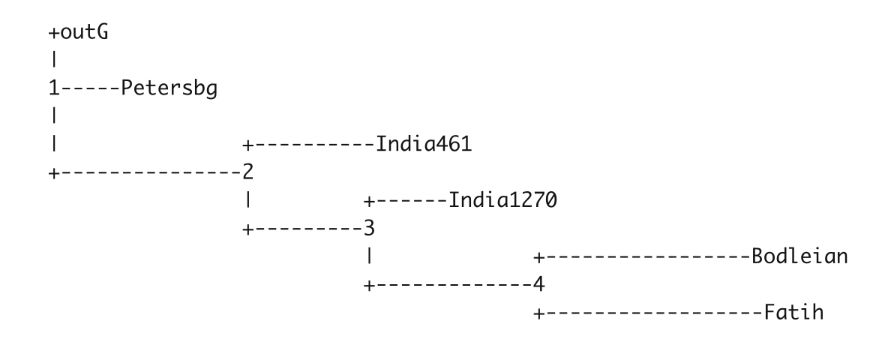
\includegraphics[width=\linewidth]{images/diagram_stemma.png}
	\end{subfigure}
	\hfill
	\begin{subfigure}{0.48\linewidth}
		\centering
		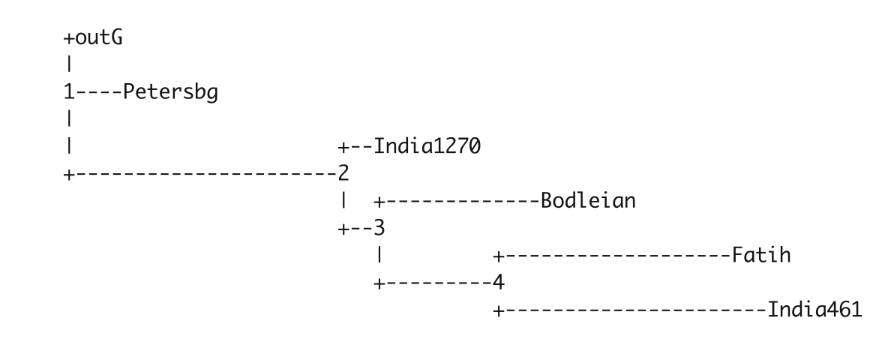
\includegraphics[width=\linewidth]{images/text_stemma.png}
	\end{subfigure}
	\caption{Stemmata pour les diagrammes (à gauche) et pour le texte (à droite) \footcite{raynaudBuildingStemmaCodicum2014}}
	\label{fig:stemma}
\end{figure}


En y regardant plus en détail, nous pouvons voir qu'il y a une forte similitude entre le \textit{stemma} textuel et le \textit{stemma} des diagrammes. Il en vient à la conclusion suivante : Quand les diagrammes sont intégrés au texte, il est envisageable de ne faire qu'un seul arbre pour les deux. Néanmoins, si les diagrammes ont été copiés a posteriori du texte ou qu'ils ont été corrigés par la suite, mieux vaut réaliser deux \textit{stemmata} distincts et étudier leur transmissions séparément. Le fait qu'ils aient été copiés par des personnes différentes à des moments différents impacte fortement leur étude. Il est même plus avantageux de réaliser le \textit{stemma codicum} d'une tradition mathématique à partir des diagrammes. La densité d'erreur serait sept à huit fois plus élevée dans un diagramme géométrique que dans un texte occupant la même superficie. Dans la mesure où sa méthode repose sur le relevé d'erreurs, il est plus judicieux de réaliser un \textit{stemma} avec des diagrammes\footcite{raynaudBuildingStemmaCodicum2014}.

Il nous est possible de retracer l'historique d'une œuvre grâce aux diagrammes. Cependant, ces derniers sont des éléments iconographiques complexes et il convient de les étudier de manière rigoureuse.


	
	\section{Limites des approches philologiques traditionnelles}
	L'historien des sciences \som{pas seulement} peut se heurter à de nombreuses difficultés lors de son étude des diagrammes. La manière de les représenter diffère en fonction des conventions et des choix éditoriaux. Comparer les diagrammes à l'œil nu devient complexe même pour un spécialiste. \som{Attention à la formulation, ce n'est pas forcément vrai et la comparaison manuelle sera toujours plus précise que le travail automatique.}

\subsection{Les différentes conventions de représentation d'un diagramme}

Le travail de l'historien des sciences peut s'avérer compliqué lorsqu'un concept ou une démonstration est représentée de manière différente dans différents témoins. \som{Non} En effet, les conventions et les choix graphiques des diagrammes diffèrent en fonction de l'époque, de l'endroit et du sujet d'étude.

Michela Malpangotto étudie ce phénomène en s'appuyant sur l'exemple de l'œuvre de Théodose les \textit{Sphériques} écrite au Ier siècle avant notre ère. Il s'agit d'un texte fondamental dans l'étude de la géométrie sphérique qui est structuré en cinquante-neuf propositions et divisé en trois livres. Il fait partie de ce que l'on nomme la \og Petite astronomie \fg, un recueil d'ouvrages compilés par les Grecs afin de faciliter la compréhension de l'\textit{Almageste} de Ptolémée. Il a été étudié et transmis pendant près de dix siècles. La géométrie sphérique est définie de la manière suivante : \og La géométrie sphérique étudie la sphère comme un objet solide mais surtout comme contexte spatial des éléments qui interagissent sur elle dans un agencement tridimensionnel complexe. \fg Il est alors nécessaire de mettre au même niveau, le plan du diagramme et l'agencement spatial des objets autour de la sphère. Cette dernière est un objet solide mais elle est surtout un contexte spatial pour des arcs, des segments de droites et des cercles qui y sont déterminés par l'intersection de différents plans inclinés dans l'agencement spatial tridimensionnel. Cependant, le concept de sphère n'est pas représenté de la même manière chez tous les auteurs \footcite{malpangottoGraphicalChoicesGeometrical2010}. 

Dans la version grecque originale, illustré ici par le manuscrit \textit{Vat. Gr. 204}, les deux parties de l'œuvre sont séparées par le choix de l'iconographie des diagrammes. Dans la première partie, nous retrouvons des diagrammes dans lesquelles la sphère n'est pas représentée. Il y a seulement des cercles produits par l'intersection du plan incliné de différentes façons qui sont représentés de manière juxtaposée dans le plan du diagrammes. Les arcs ainsi que les segments linaires sont aplatis et les objets placés de l'autre côté de la sphère sont retournés dans le plan de la figure. La conséquence majeure de ce mode de représentation est la dépendance des diagrammes vis-à-vis du texte. Il est nécessaire de lire les explications pour comprendre le diagramme. Dans la seconde partie de l'œuvre, les diagrammes sont construits en utilisant la perspective. Nous pouvons donc observer les éléments géométriques interagir entre eux à l'intérieur de cette dernière \footcite{malpangottoGraphicalChoicesGeometrical2010}.  

En Italie, Platon de Tivoli a réalisé trois éditions de cette œuvre au XVIe siècle en s'appuyant sur une version arabo-latine médiévale. Il choisit de représenter les diagrammes de manière schématique et plane comme dans la première partie de la version grecque originale de l'œuvre. L'édition de Francesco Maurolico marque un tournant dans la transmission des \textit{Sphériques}. En effet, ce dernier fait le choix de travailler sur la surface de la sphère qui, mise en avant, devient le contexte réel dans lequel les éléments géométriques interagissent. Christophe Clavius, un mathématicien allemand adopte cette iconographie dans son édition de 1586 qui sert de base à la tradition moderne des \textit{Sphériques}\footcite{malpangottoGraphicalChoicesGeometrical2010}. 

\begin{figure}[H]
	\centering
	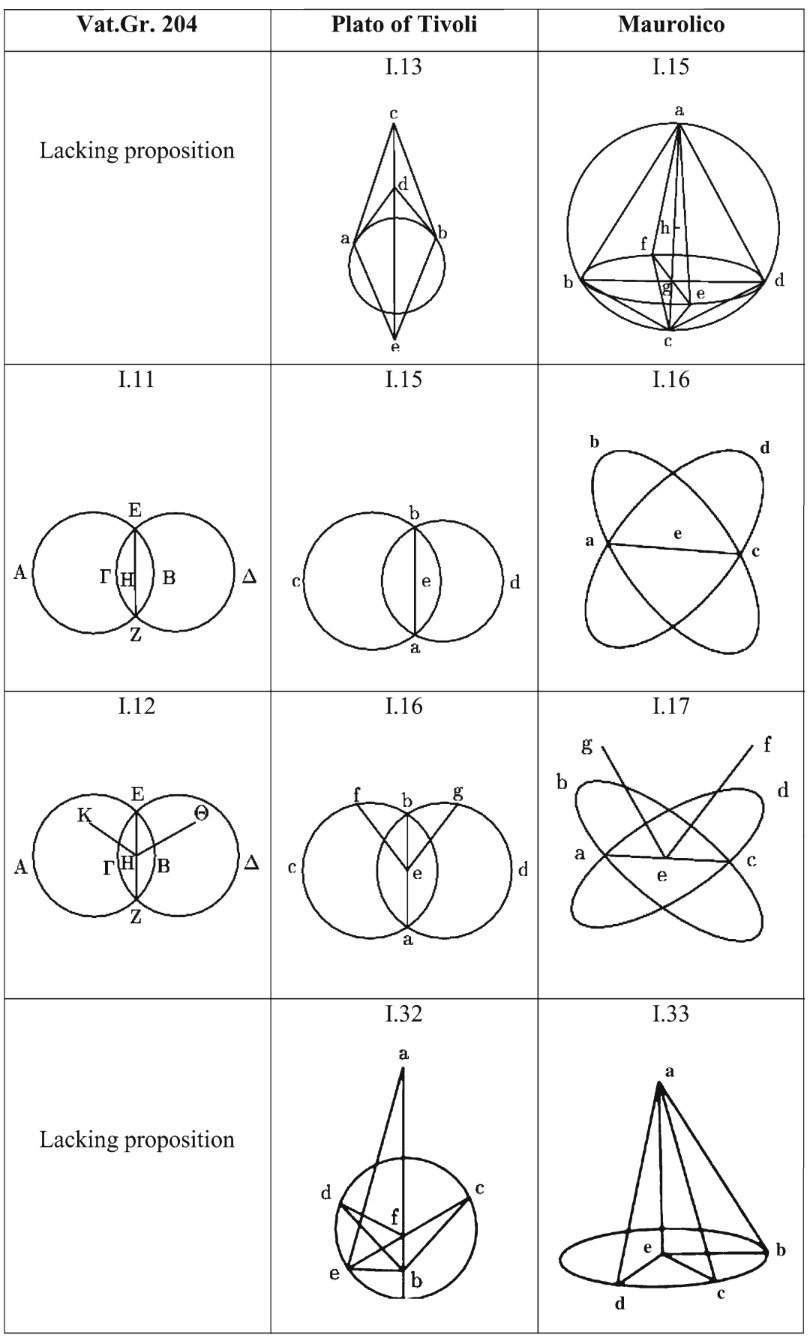
\includegraphics[width=0.6\linewidth]{images/conventions_diagrammes.png}
	\caption{Différentes conventions de représentation de diagrammes évoquées par Michela Malpangotto\footcite{malpangottoGraphicalChoicesGeometrical2010}}
	\label{fig:conventions}
\end{figure}


L'étude de Michela Malpangotto nous montre l'existence de nombreuses conventions graphiques de diagrammes pouvant être très différentes en fonction des éditeurs et des époques. Lorsque nous tentons de retracer la diffusion d'une œuvre à partir de ces diagrammes, il est important de prendre en compte ce paramètre. Néanmoins, ces différentes manières de représenter les diagrammes sont aussi en elles-mêmes les témoins de l'évolution d'un concept et donc par extension des connaissances scientifiques. \\

La question de la représentation des diagrammes est aussi une problématique que nous retrouvons dans les éditions plus contemporaines. 

\som{Mais du coup, les travaux cités comme exemple ont bel et bien été faits manuellement, sans que cela ne présente de difficulté particulière pour les chercheurs. Je pense que cette partie tombe à côté de la véritable problématique du projet, càd qu'il existe à travers les traditions un très grand nombre de manuscrits, qu'il est impossible sur le temps d'une vie de tous comparer précisément. De même, la question de la langue est importante, puisque c'est ça qui pose problème aux chercheurs qui sont rarement spécialistes de toutes les langues à la fois, et n'ont dans ce cas pas les outils pour faire des comparaisons à travers les traditions. Cela n'a rien à voir avec les conventions de représentation des diagrammes en elles-mêmes, d'autant qu'un outil numérique ne peut pas non plus faire cette comparaison automatiquement. On questionne donc la pertinence de l'argumentaire pour répondre à la problématique.}

\subsection{La modification des diagrammes dans les éditions modernes des sources scientifiques}

Les modifications que s'autorisent à faire les historiens et éditeurs contemporains peuvent rendre la comparaison avec les sources anciennes compliquée. Dans l'article déjà cité précédemment, Ken Saito étudie les éditions modernes des diagrammes astronomiques des \textit{Elements} d'Euclide. Il expose la problématique suivante : les diagrammes que nous voyons dans les éditions imprimées à partir du XIXe siècle sont très différents de ceux présents dans les manuscrits médiévaux. Pourtant les témoins datant du Moyen Age sont les meilleures versions, voire les seuls exemplaires d'œuvres antiques mathématiques en absence de manuscrit datant de cette époque. La version qui sert de base à beaucoup d'éditions contemporaines est celle de Heiberg datant de 1883-1888. Cependant, ce dernier s'est contenté de recopier les diagrammes de Ferdinand August simplifiés dans un but pédagogique dans son édition datant des années 1820 \footcite{saitoTraditionsDiagramTradition2012}. Se pose alors la question des conventions d'édition. Deux points de vue s'opposent. Nous avons d'abord celui de la maison d'édition \textit{Les Belles Lettres} décrit dans leur \textit{Règles et recommandations pour les éditions critiques} qui explique qu'il est nécessaire de reproduire les diagrammes aussi précisément que possible sans essayer de les corriger ou de les modifier. Michael Hunter, lui, défend plutôt l'idée selon laquelle il est acceptable que les diagrammes soient redessinés pour que l'intention originelle de l'auteur soit transmise au lecteur\footcite{jardineCriticalEditingEarlyModern2010}.\\

Ces différentes manières de représenter un même diagramme peuvent poser problème aux chercheurs lorsque ces derniers cherchent à établir des liens entre les différents témoins d'une même œuvre ou tradition. Même pour un spécialiste qui connaît parfaitement les différentes conventions, identifier et comparer chaque diagramme dans plusieurs témoins peut s'avérer être très chronophage.

\som{Pourquoi on voudrait comparer sources anciennes et contemporaines ? Ce n'est le sujet d'aucun projet de recherche cités dans le mémoire, et encore une fois, un chercheur qui le souhaite peut tout à fait faire cette comparaison. Ça n'a rien à voir avec les modifications que font les éditeurs et les historiens. Ce que AIKON/EIDA questionne, c'est l'absence de normes d'édition et de vocabulaire standardisé pour l'édition des diagrammes.}
	
	
	
	\clearemptydoublepage
	
	\chapter{AIKON et l'automatisation des traitements}
	
	\section[La plateforme AIKON]{Le choix de la vision artificielle pour ces objets d'étude : la plateforme AIKON}
	
		La vision artificielle ou computer vision en anglais est \og une branche spécifique de l'intelligence artificielle traitant de l'acquisition par une machine de compétences de traitement et d'analyse d'image numériques pour en extraire des données \fg \footcite{norindrTraitementSourcesHistoriques2023}.
	Dans le cadre de l'application AIKON, la vision artificielle n'a pas pour ambition de remplacer les historiens mais de faciliter leur travail de recherche à l'aide d'outils développés pour répondre aux besoins spécifiques des sciences historiques. 
	La vision artificielle a déjà beaucoup été exploitée dans le domaine des sciences historiques et de la philologie pour traiter des données textuelles, notamment avec l'\gls{ocr} et l'\gls{htr}. Cependant, elle reste encore trop souvent peu exploitée pour le traitement automatique des images dans ces disciplines.

\subsection{Avant AIKON : le projet EnHerit}

\gls{enherit}\footcite{EnHeritEnhancingHeritage} est un projet ANR porté par l'Ecole nationale des ponts et chaussées qui s'est déroulé entre 2018 et 2023.

Ce projet a pour objectif d'isoler des \textit{patterns} récurrents dans plusieurs documents iconographiques pour tracer des liens entre ces derniers.

Les chercheurs du projet ont choisi de travailler sur un \textit{dataset} de 1587 œuvres attribuées à Jan Brueghel et son atelier. Contrairement à ce que nous pourrions penser, les œuvres d'art produites dans ce type de contexte ne sont pas toutes uniques. Il est fréquent que des croquis préliminaires et des études soient dupliquées et réutilisés sur d'autres œuvres. Cependant, reconnaître les motifs et faire des liens entre les différentes œuvres n'est pas une tâche évidente, notamment à cause de la diversité des techniques utilisées comme la peinture à l'huile, le pastel ou le dessin par exemple. A travers ce \textit{dataset}, l'équipe du projet \gls{enherit} cherche à extraire des \textit{patterns} récurrents et à réaliser des connexions visuelles entre les différentes œuvres de l'atelier de Jan Brueghel. Les outils développés à partir de ce \textit{dataset} permettent aux historiens de l'art de réaliser une tâche qu'auparavant ils accomplissaient à la main. En effet, ces avancées ont pour but de remplacer la collation manuelle des images durant laquelle les historiens de l'art traçaient à la main chaque motif pour ensuite les comparer. Dans le cas du \textit{dataset} de l'atelier de Jan Brueghel, cela représenterait plusieurs années de travail.

\begin{figure}[h]
	\centering
	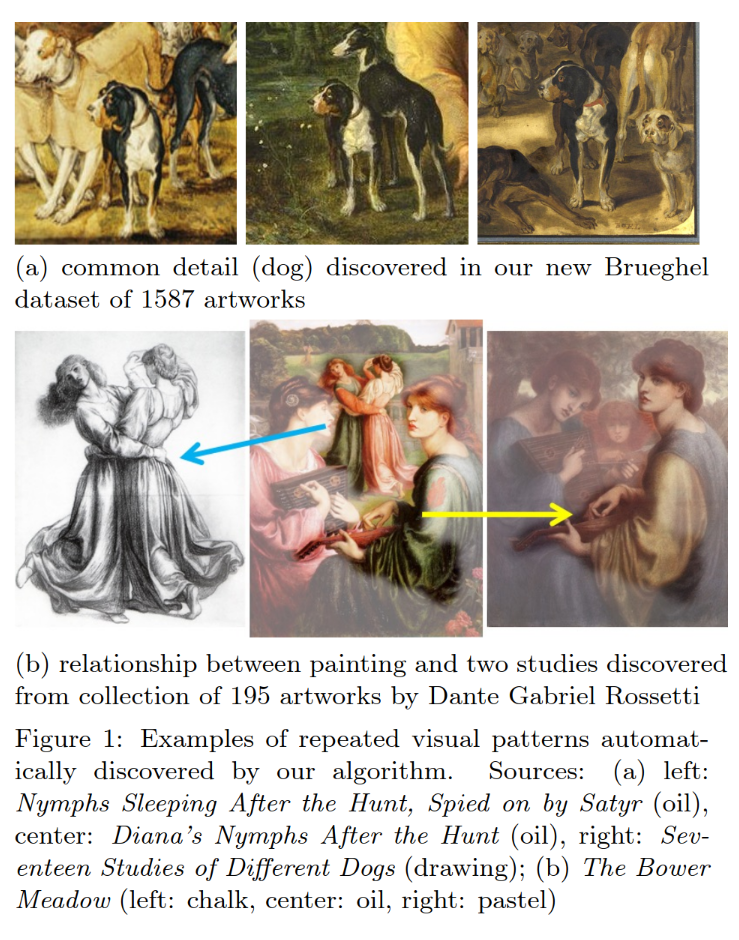
\includegraphics[width=0.7\linewidth]{images/exemples_patterns_enherit.png}
	\caption{Exemples de \textit{patterns} répétés dans plusieurs œuvre issues du data de Jan Brueghel \footcite{shenDiscoveringVisualPatterns2019}}
	\label{fig:exemples_patterns_repetes}
\end{figure}

Cependant, l'un des problèmes que nous pouvons rencontrer dans ce type de projet est l'annotation manuelle qui peut se révéler fastidieux pour les historiens de l'art. C'est pour cette raison, que les chercheurs du projet \gls{enherit} ont choisi d'utiliser l'apprentissage auto-supervisé aussi appelé \textit{self-supervised learning}\footcite{shenDiscoveringVisualPatterns2019}.
L'apprentissage auto-supervisé est \og une technique de \textit{machine learning} qui utilise l'apprentissage non-supervisé pour des tâches qui, habituellement, nécessitent un apprentissage supervisé \fg. Dans le cadre de l'apprentissage supervisé, il est nécessaire d'annoter les données au préalable tandis que dans l'apprentissage non supervisé, un algorithme les génère tout seul\footcite{QuestceQueLapprentissage2023}.
Pour effectuer cette tâche, il est nécessaire au préalable de réaliser un apprentissage des caractéristiques. Il faut d'abord échantillonner un \textit{patch} pour trouver des candidats. Ensuite, nous filtrons les faux positifs par le biais de la cohérence spatiale avant de mettre en place un apprentissage métrique avec des paires positives et négatives. C'est de cette manière que l'outil ArtMiner a été développé\footcite{ArtMiner}. Ce dernier est réutilisé par la suite par le projet \gls{vhs}. 
L'algorithme Segswap disponible dans l'application AIKON est également issu de ce projet.

A partir des avancées réalisées dans le cadre de \gls{enherit}, un autre projet est né : le projet AIKON.

\subsection{L'application AIKON}

\subsubsection{Présentation}
AIKON est une application de recherche conçue pour permettre aux chercheurs en Sciences Humaines et Sociales d'exploiter des outils de computer vision afin d'analyser de vastes corpus de données historiques\footcite{aikonAikonplatformAikon2025}. 
Sa plateforme mais aussi les modèles d'intelligence artificielle disponibles dessus sont tous \textit{open source}. Cela signifie que n'importe qui peut accéder au code et utiliser l'application de manière gratuite. Elle est donc à la fois accessible à de gros projet mais aussi à des chercheurs qui l'utiliseraient pour des projets personnels. 
AIKON permet de décrire les sources historiques et analyser des corpus visuels en vue de leur potentielle édition\footcite{albouyAIKONComputerVision}.

\subsubsection{L'architecture}

L'architecture de l'application AIKON est la même pour tous les projets qui l'utilisent.

\begin{figure}[H]
	\centering
	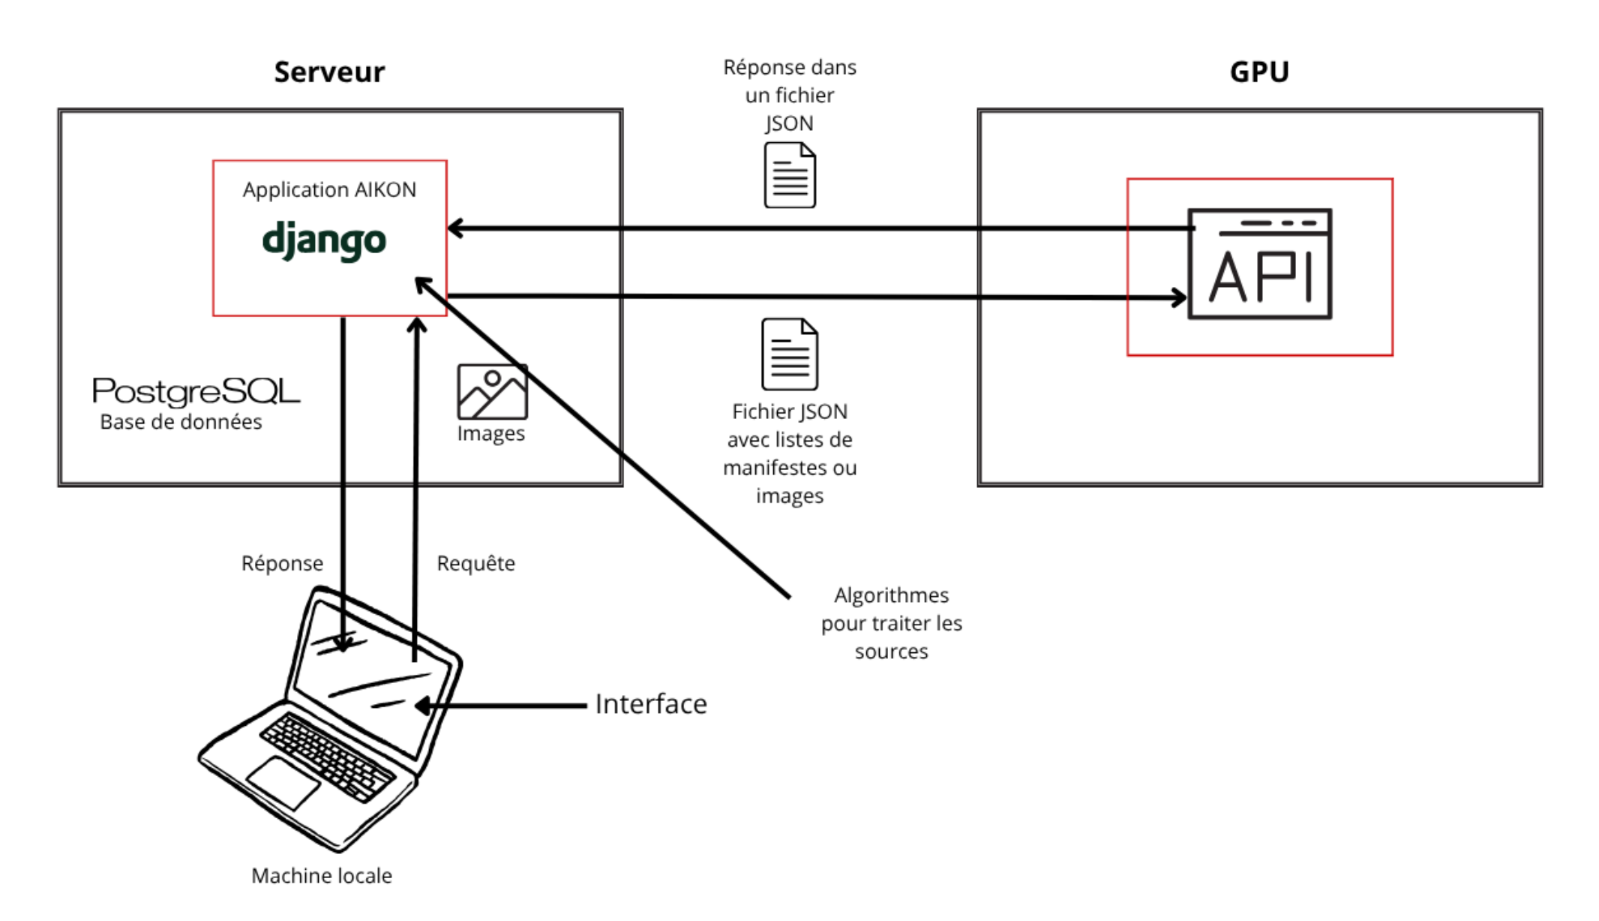
\includegraphics[width=1\textwidth]{images/architecture_aikon.png}
	\caption{Architecture de l'application AIKON}
	\label{fig:architecture_aikon}
\end{figure}

L'utilisateur interagit avec l'application via une interface graphique. Il envoie une requête à l'application qui est stockée sur un serveur. Par exemple, la plateforme \gls{eida} est hébergée sur le serveur Syrte9 de l'Observatoire de Paris. AIKON est codée en python avec Django. Il s'agit d'un \textit{framework} \textit{open-source} qui permet de développer des applications web robustes facilement. Sur le serveur, il y a également la base de données PostgreSQL et les numérisations du projet. Pour réaliser un traitement automatique des données, l'extraction de regions ou la reconnaissance de similarités par exemple, l'application convertit la numérisation du document en manifeste \gls{iiif}. Un manifeste \gls{iiif} est un fichier qui décrit la structure et le contenu d'un document numérisé pour permettre son affichage et son interaction sur le web. Ce fichier est envoyé à l'\gls{api} stockée au sein d'un \gls{gpu}, un processeur spécialisé conçu pour manipuler et afficher rapidement des images. Lorsque l'\gls{api} reçoit le manifeste \gls{iiif}, elle traite le fichier avec l'algorithme choisit par l'utilisateur via l'interface graphique. Ensuite, l'\gls{api} renvoie un fichier .txt avec des annotations à l'application. Pour finir, l'utilisateur peut accéder aux résultats de l'opération sur son interface graphique pour les utiliser.

\subsubsection{Le modèle de données}

AIKON possède un modèle de données commun à tous les projets qui l'exploitent. Ce dernier est composé de plusieurs tables connectées entre elles.

\begin{figure}[H]
	\centering
	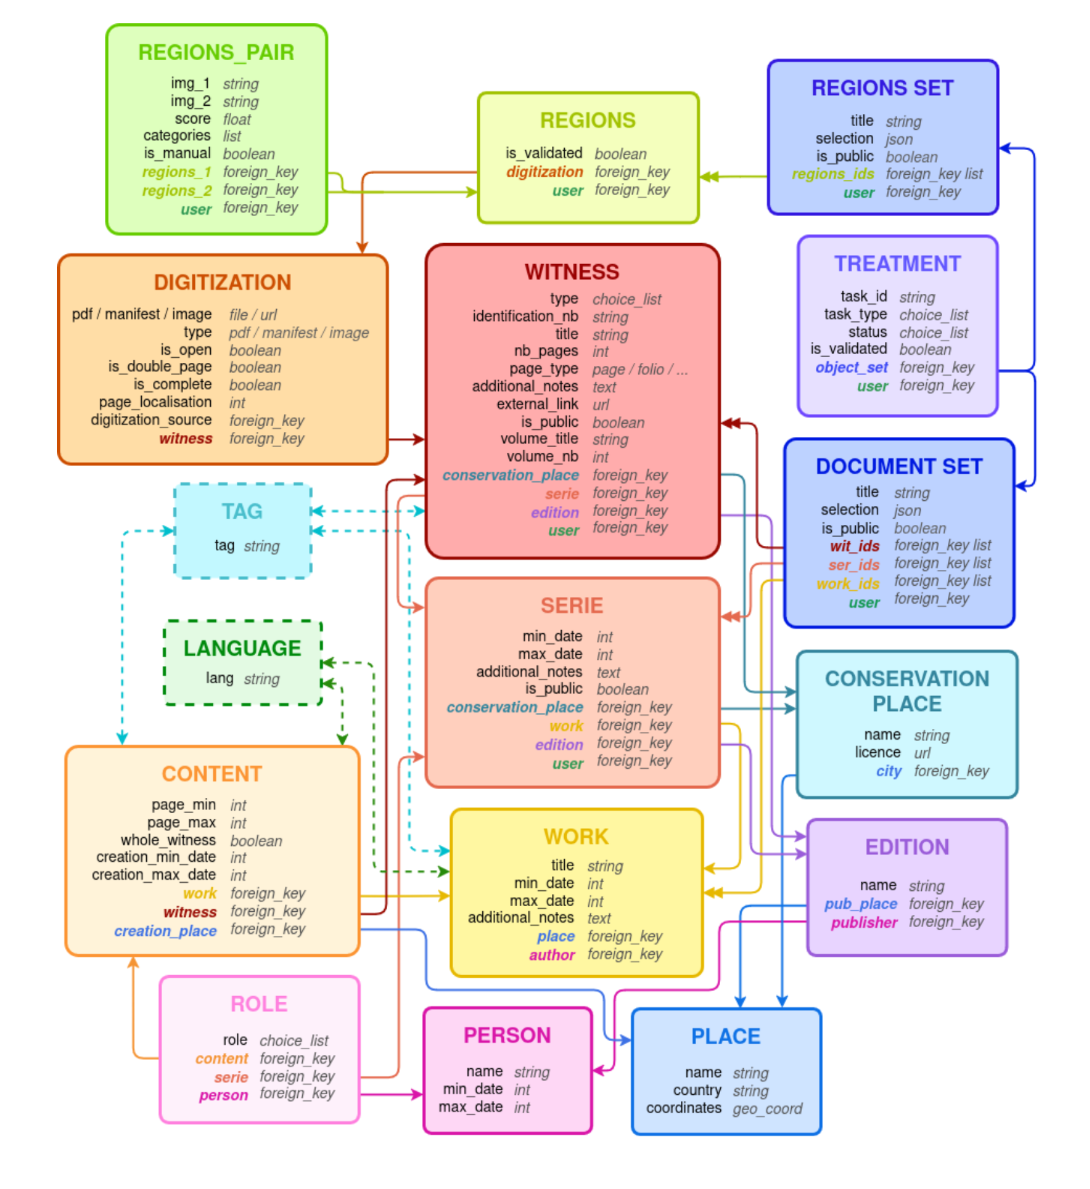
\includegraphics[width=1\textwidth]{images/modele_donnees_aikon.png}
	\caption{Modèle de données de l'application AIKON}
	\label{fig:modele_donnees}
\end{figure}

La table centrale du modèle de données est \textit{witness}. Elle contient toutes les informations relatives à chaque document numérisé mis en ligne sur l'application. Elle est reliée aux autres tables par le biais de \textit{foreign keys}. 

Dans ce modèle de données, nous retrouvons des tables reliées à des fonctions différentes : 
\begin{itemize}
	\item La description du \textit{witness} et de ses métadonnées : \textit{witness, conservation place, edition, place, person, role, content, language}
	\item La numérisation du \textit{witness} : \textit{digitization}
	\item L'organisation des \textit{witnesses} en clusters : \textit{serie, document set}
	\item : Les traitements automatiques : \textit{treatment, regions set, regions, region pairs} 
\end{itemize}

Evidemment ces fonctions ne sont pas hermétiques car les tables sont toutes reliées entre elles.

\begin{figure}[H]
	\centering
	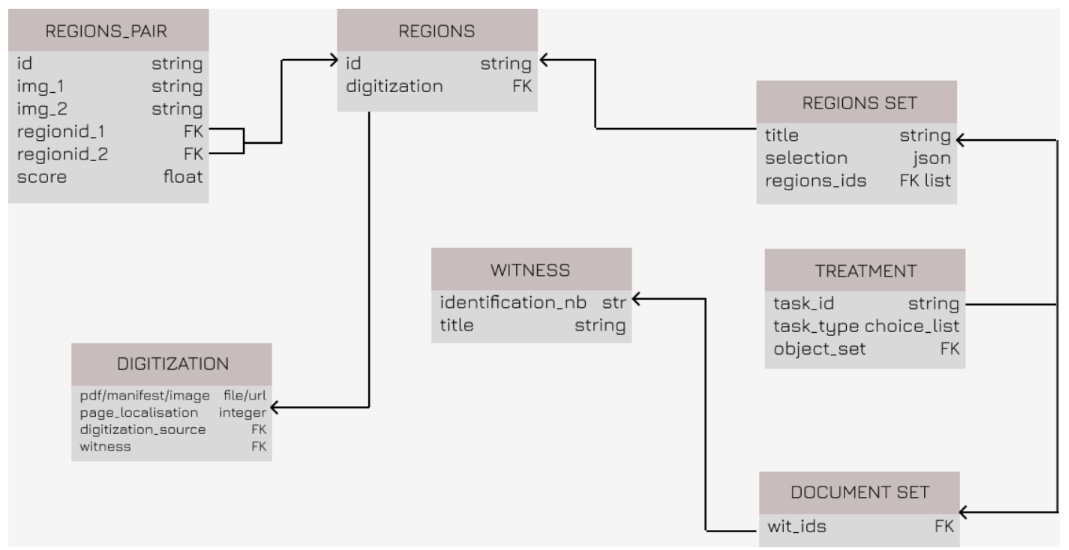
\includegraphics[width=1\textwidth]{images/tables_traitement_donnees.png}
	\caption{Tables en lien avec le traitement automatique des données}
	\label{fig:tables_traitement}
\end{figure}

Dans le cadre de notre étude, nous allons surtout nous concentrer sur les tables relatives au traitement automatique des sources et notamment à region pairs. \\

L'application AIKON est actuellement utilisée par deux projet : \gls{eida} et \gls{vhs}.

\subsection{Le projet VHS}

\gls{vhs} est un projet qui a pour but de mettre en place une nouvelle approche de l'étude historiques du savoir scientifique en utilisant les outils numériques pour l'analyse d'image. Il rassemble trois équipes de recherche : l'équipe Digital Humanities de l'Institut des Sciences du Calcul et des Données de Sorbonne Université, l'équipe Monde Byzantin du laboratoire Orient et Méditerranée (UMR 8167) et l'équipe IMAGINE du Laboratoire d'informatique Gaspard Monge de l'Ecole nationale des Ponts et Chaussées\footcite{Presentation}.* Carnet Hypothèse VHS Il a permis de constituer un nouveau \textit{dataset} d'illustrations scientifiques du Moyen-Age et de l'époque moderne. Cela a permis d'extraire près de 235000 images à partir de 405000 pages du corpus. Suite à l'annotation manuelle des résultats d'extraction d'image, 8000 d'entre-elles ont été validées par des historiens\footcite{fouadComputerVisionHistorical2023}. Ce \textit{dataset} est composé de quatre corpus sélectionnés pour leur diversité en ce qui concerne leur thématique, leur époque et leur aire géographique. 
Nous avons d'abord le \textit{Physiologus} un texte rédigé vers le IIe siècle de notre ère à Alexandrie. Il est composé d'une centaine de manuscrits écrits en grec dont 13 d'entre eux sont illustrés. Ces derniers ont été réalisés entre le XIe et le XVIe siècle et ils ont été diffusés dans tout l'Occident chrétien. Nous avons pu extraire environ 680 images d'animaux, de plantes et de minéraux. 
Le deuxième corpus concerne le \textit{De materia medica} écrit vers 77 de notre ère par Dioscoride. Il est conservé dans 65 manuscrits grecs. 17 d'entre eux réalisées entre le VIe et le XVIe siècle sont illustrés d'environ 8340 images de plantes, d'animaux et de minéraux. 
Les deux derniers corpus contiennent des planches de \textit{l'Encyclopédie} de Diderot et d'Alembert publiées entre 1751 et 1772 mais aussi leurs sources et leur inclusion ultérieure dans d'autres encyclopédies. Les deux thèmes principaux de ces corpus sont l'histoire naturelle et les sciences mathématiques. 
Ainsi, nous retrouvons au sein du projet \gls{vhs} à la fois deux œuvres datant de l'Antiquité et ayant été diffusés durant tout le Moyen Age et l'époque moderne dans tout l'Occident mais aussi une œuvre plus tardive qu'est \textit{l'Encyclopédie} de Diderot et d'Alembert qui a également eu une grande influence notamment dans l'écriture d'encyclopédies postérieures\footcite{Corpus}.* VHS Hypothèses (corpus)



\subsection{Le projet EIDA}

\gls{eida} est un projet ANR PRC d'envergure internationale qui a pour but l'étude et l'analyse des diagrammes de tradition ptolémaïque dans un corpus de témoins allant du IXe siècle au XIXe siècle avec des sources en latin, hébreu, sanskrit, byzantin, perse, grec, chinois et arabe. Il rassemble deux équipes de recherche. Le laboratoire \gls{lte} de l'Observatoire de Paris s'occupe principalement de la partie histoire des sciences du projet tandis que l'équipe IMAGINE de l'Ecole nationale des Ponts et Chaussées gère la partie \textit{computer vision}\footcite{albouyAIKONComputerVision}. 

Le but du projet serait de développer des outils pour que les chercheurs puissent explorer, visualiser le corpus, communiquer les résultats lors de conférences et réaliser des éditions de diagrammes nativement numériques \footcite{Conference2023EIDA2023}.

Le projet encore en cours s'est déroulé en plusieurs étapes. La première concernait la constitution du corpus. Les chercheurs cherchent à étudier le diagramme sous un angle documentaire en tant que artefact et sous son angle épistémique en tant qu'outil de compréhension pour les acteurs historiques\footcite{Conference2023EIDA2023}.

Suite au développement des premiers outils numériques de la plateforme, il a été possible d'appliquer aux sources de premiers traitements automatiques. L'extraction puis la reconnaissance automatique de \textit{region pairs} et le calcul de similarité ont permis de distinguer les diagrammes en double et de les interpréter dans plusieurs traditions, œuvres et témoins\footcite{Conference2024Graphic2024}.

Les chercheurs ont pu réaliser de premières observations. Il se trouve que les diagrammes peuvent être regroupés en fonction de leurs similarités. Un diagramme peut être rattaché à une œuvre, à une thématique ou à une famille\footcite{Conference2025Long2025}. 

Les chercheurs se réunissent régulièrement pour mener une réflexion autour du projet lors de conférences et séminaires. 
 

Sur le long terme, le but du projet serait de mettre à disposition des chercheurs une interface utilisateur sur le modèle de celle de \gls{dishas}, un projet antérieur mené par l'Observatoire de Paris. \\

D'autres projets ont souhaiteraient utiliser AIKON à l'avenir pour traiter leurs sources. C'est le cas du projet ANR High Vision dont le but est d'étudier en s'aidant de la \textit{computer vision} des photographies de presse datant de la fin XIXe siècle au début du XXe siècle qui ont été numérisées en masse. * carnet hypthèse High Vision



  
	


	
	\section{Les fonctionnalités de computer vision dans AIKON}
	\subsection{L'extraction des regions}

Il existe plusieurs algorithmes pour extraire des \textit{regions} \som{Tu peux dire "régions", ça fera plus propre !} dans AIKON. 
Pour l'extraction des diagrammes astronomiques du projet EIDA, nous retrouvons l'algorithme \textit{Diagram extraction (YOLO model fine-tuned on historical diagrams)}.
Pour VHS, nous avons l'algorithme \textit{Illustration extraction (YOLO model fine-tuned on historical illustrations)}. Ce dernier a été entraîné dans le cadre du projet \gls{enherit} cité précédemment. JE NE COMPRENDS PAS

\som{VHS et EIDA n'utilisent pas de modèles différents à proprement parler, et aucun des deux projets n'utilise un algo d'extraction entraîné par EnHerit. Les deux projets utilisent des versions fine-tunée (réentraînées) de YOLO, qui ont été entraînées sur des données synthétiques, puis sur les données de VHS (ils s'arrêtent là de leur côté), puis sur les données d'EIDA. Ainsi, on évite de démultiplier les entraînements qui nécessitent beaucoup d'annotations.}

\subsection{La reconnaissance et le calcul de similarité}

\subsubsection{La collation des images}

La collation dans le domaine de la philologie désigne l'action de comparer plusieurs témoins d'une même œuvre pour relever leurs différences et leurs similitudes. 

Il existe déjà des outils pour collationner les textes automatiquement depuis longtemps. A la fin des années 1940, Charlton Hinman avait déjà créer une machine nommée le collationneur Hinman ou Hinman Collator en anglais pour collationner des impressions du \textit{Premier Folio} de William Shakespeare. Plus récemment, le logiciel CollateX permet de comparer des versions numériques du texte automatiquement\footcite{kaouaImageCollationMatching2021}. 

Néanmoins, ces outils ne sont pas transposables sur les éléments iconographiques. Les méthodes d'alignement de texte avec transcription et la tokenisation \som{Expliquer en nbp} utilisées sur les textes ne sont pas applicables aux images\footcite{kaouaImageCollationMatching2021}. C'est pour cette raison que les chercheurs du projet AIKON ont développé des algorithmes de reconnaissance et de calcul des similarités.

\som{Vrai en partie, le but plus exact est de retrouver des copies d'un même motif dans un vaste corpus, cf VHS qui s'intéresse à la réutilisation de planches de l'Encyclopédie. Pour moi, la présentation et l'explication des projets doit s'insérer à ce genre de partie pour expliciter le propos.} 


\subsubsection{Les algorithmes présents sur AIKON}

L'algorithme utilisé pour reconnaître automatiquement les similarités et calculer leur score est SegSwap qui a notamment été entraîné sur le \textit{dataset} de Brueghel cité plus haut. \som{SegSwap a été entraîné sur un jeu de données synthétique. Je pense dans tous les cas qu'il n'est pas nécessaire de se focaliser sur les algorithmes et leur entraînement, vu que ce n'est pas le sujet du stage.} Il a également été testé sur deux autres \textit{datasets} d'images représentant des images de scènes urbaines (citer les noms). Il commence par extraire des segments significatifs sur les images. Ensuite, il copie le segment d'une image A sur une image B pour créer une image modifiée synthétique contenant le segment natif et le segment de l'autre image \som{Ce processus est celui utilisé pour générer des données d'entraînement synthétique, du coup.}. Le but est de reconnaître les morceaux d'image copiés entre les deux images et ignorer les zones non modifiées.  Il s'agit d'apprentissage automatique donc il n'a pas besoin d'annotation, il en génère tout seul \footcite{shenLearningCosegmentationSegment2022} vérifier. 

\som{Je pense qu'il n'est pas nécessaire de s'étendre autant du SegSwap, surtout après en avoir parlé plus tôt pour EnHerit. Selon moi, la mention d'EnHerit devrait venir en même temps que l'explication de SegSwap, comme exemple d'utilisation. Cependant, vu le sujet du mémoire, je ne sais pas si c'est bien nécessaire.} 

	
	\section[Les interfaces existantes]{De l'annotation manuelle au traitement de masse : les interfaces existantes}
	Les différents projets utilisant AIKON possèdent leur propre interface avec des bases de données distinctes hébergés sur des serveurs différents. Cependant, son aspect et son fonctionnement restent les mêmes.

\begin{figure}[h]
	\centering
	\begin{subfigure}{0.48\linewidth}
		\centering
		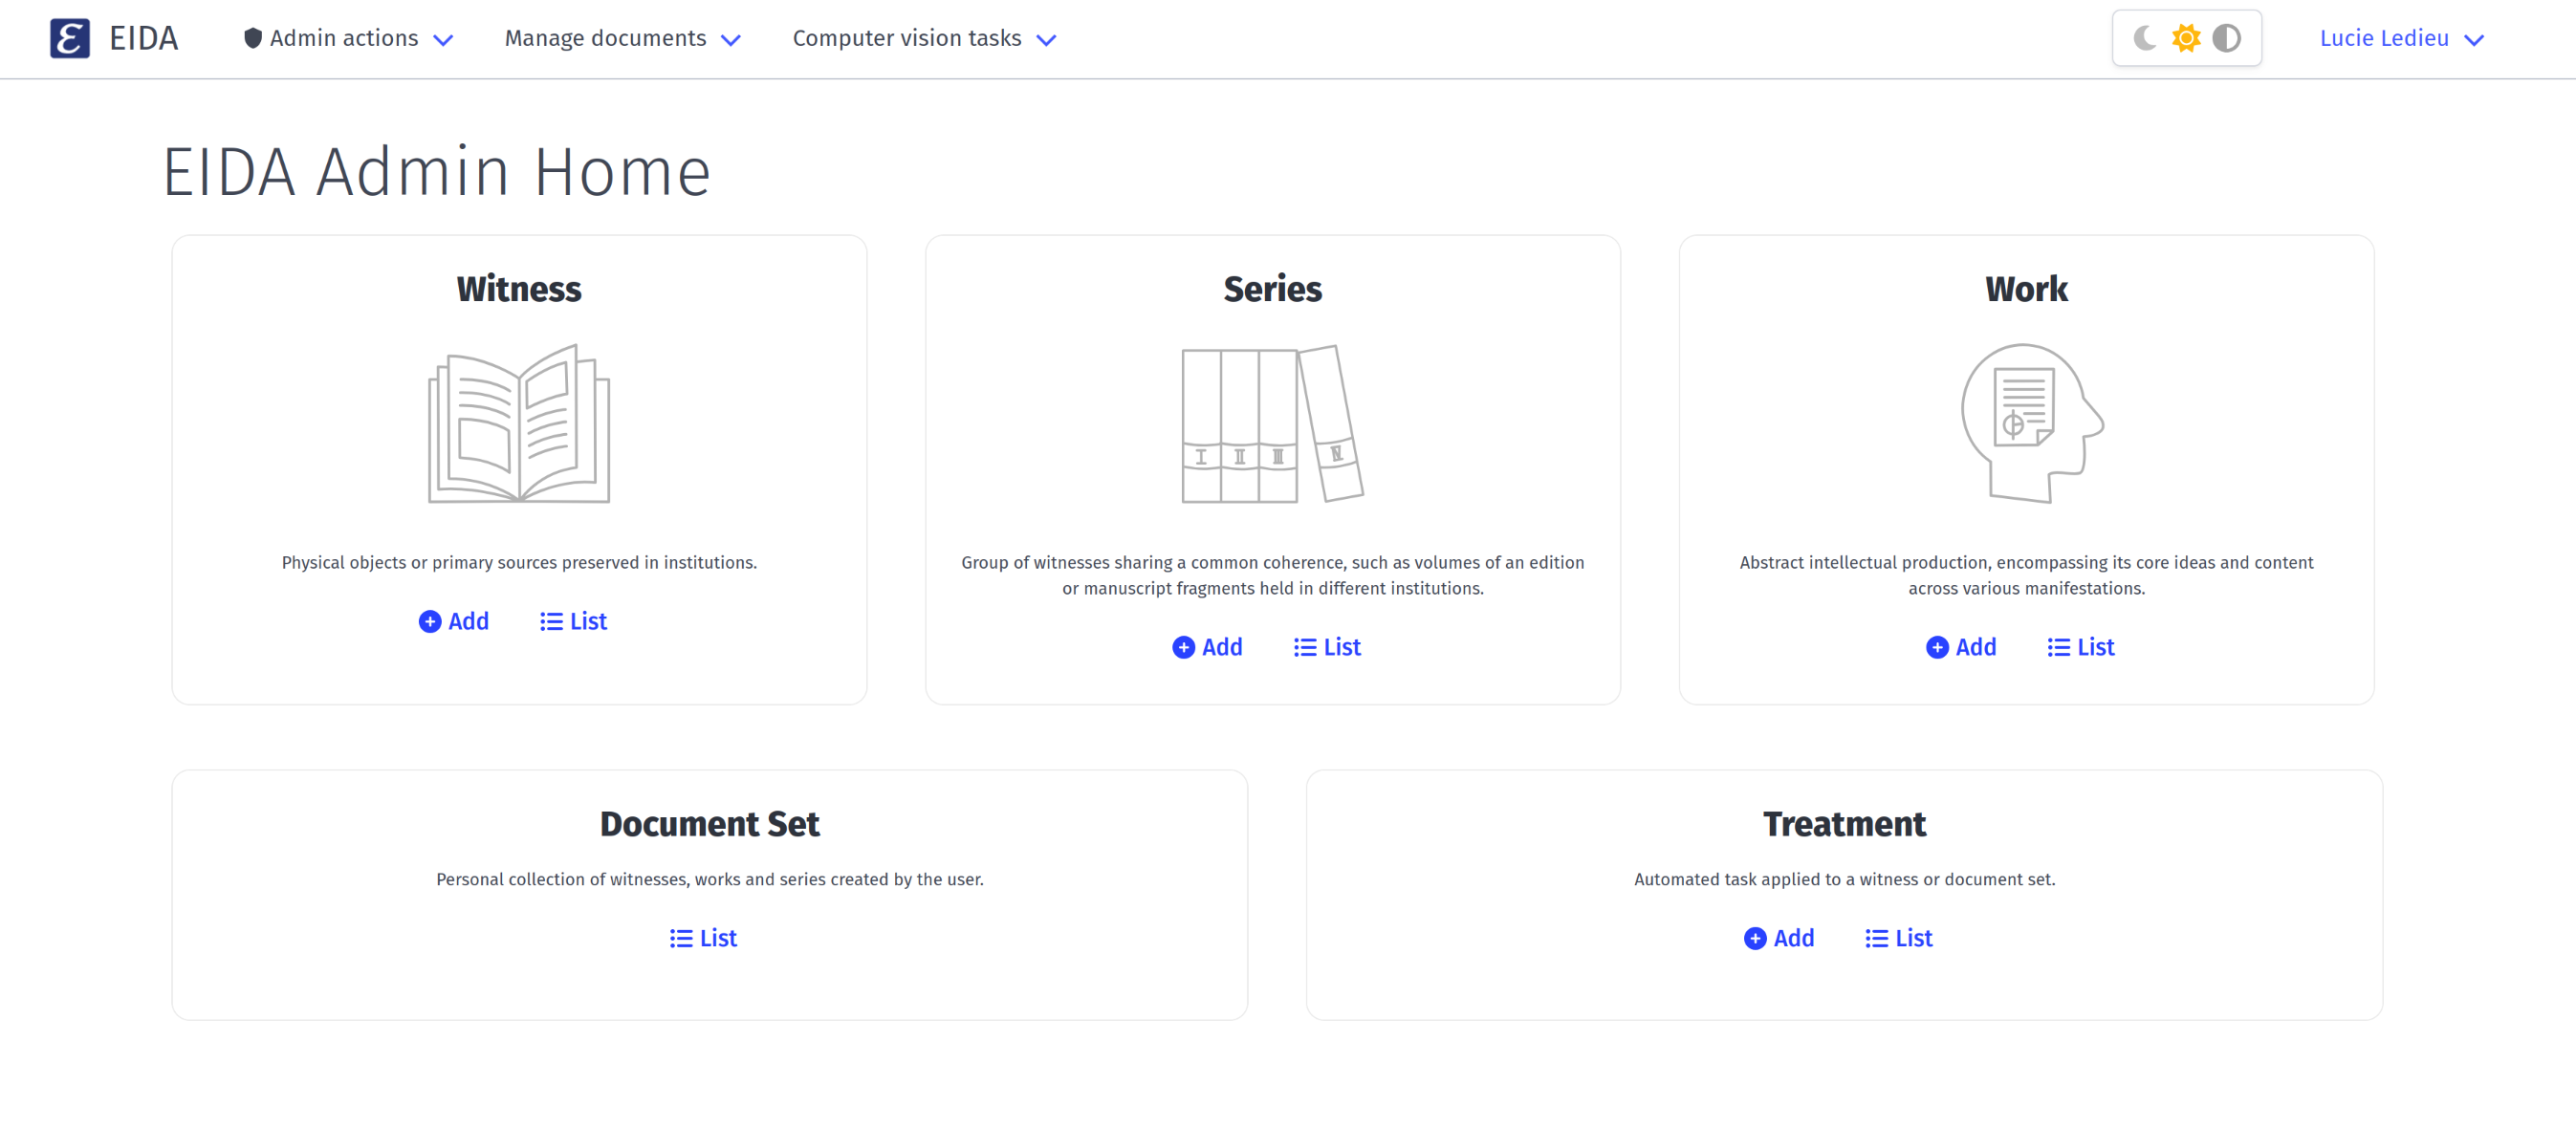
\includegraphics[width=\linewidth]{images/accueil_eida.png}
	\end{subfigure}
	\hfill
	\begin{subfigure}{0.48\linewidth}
		\centering
		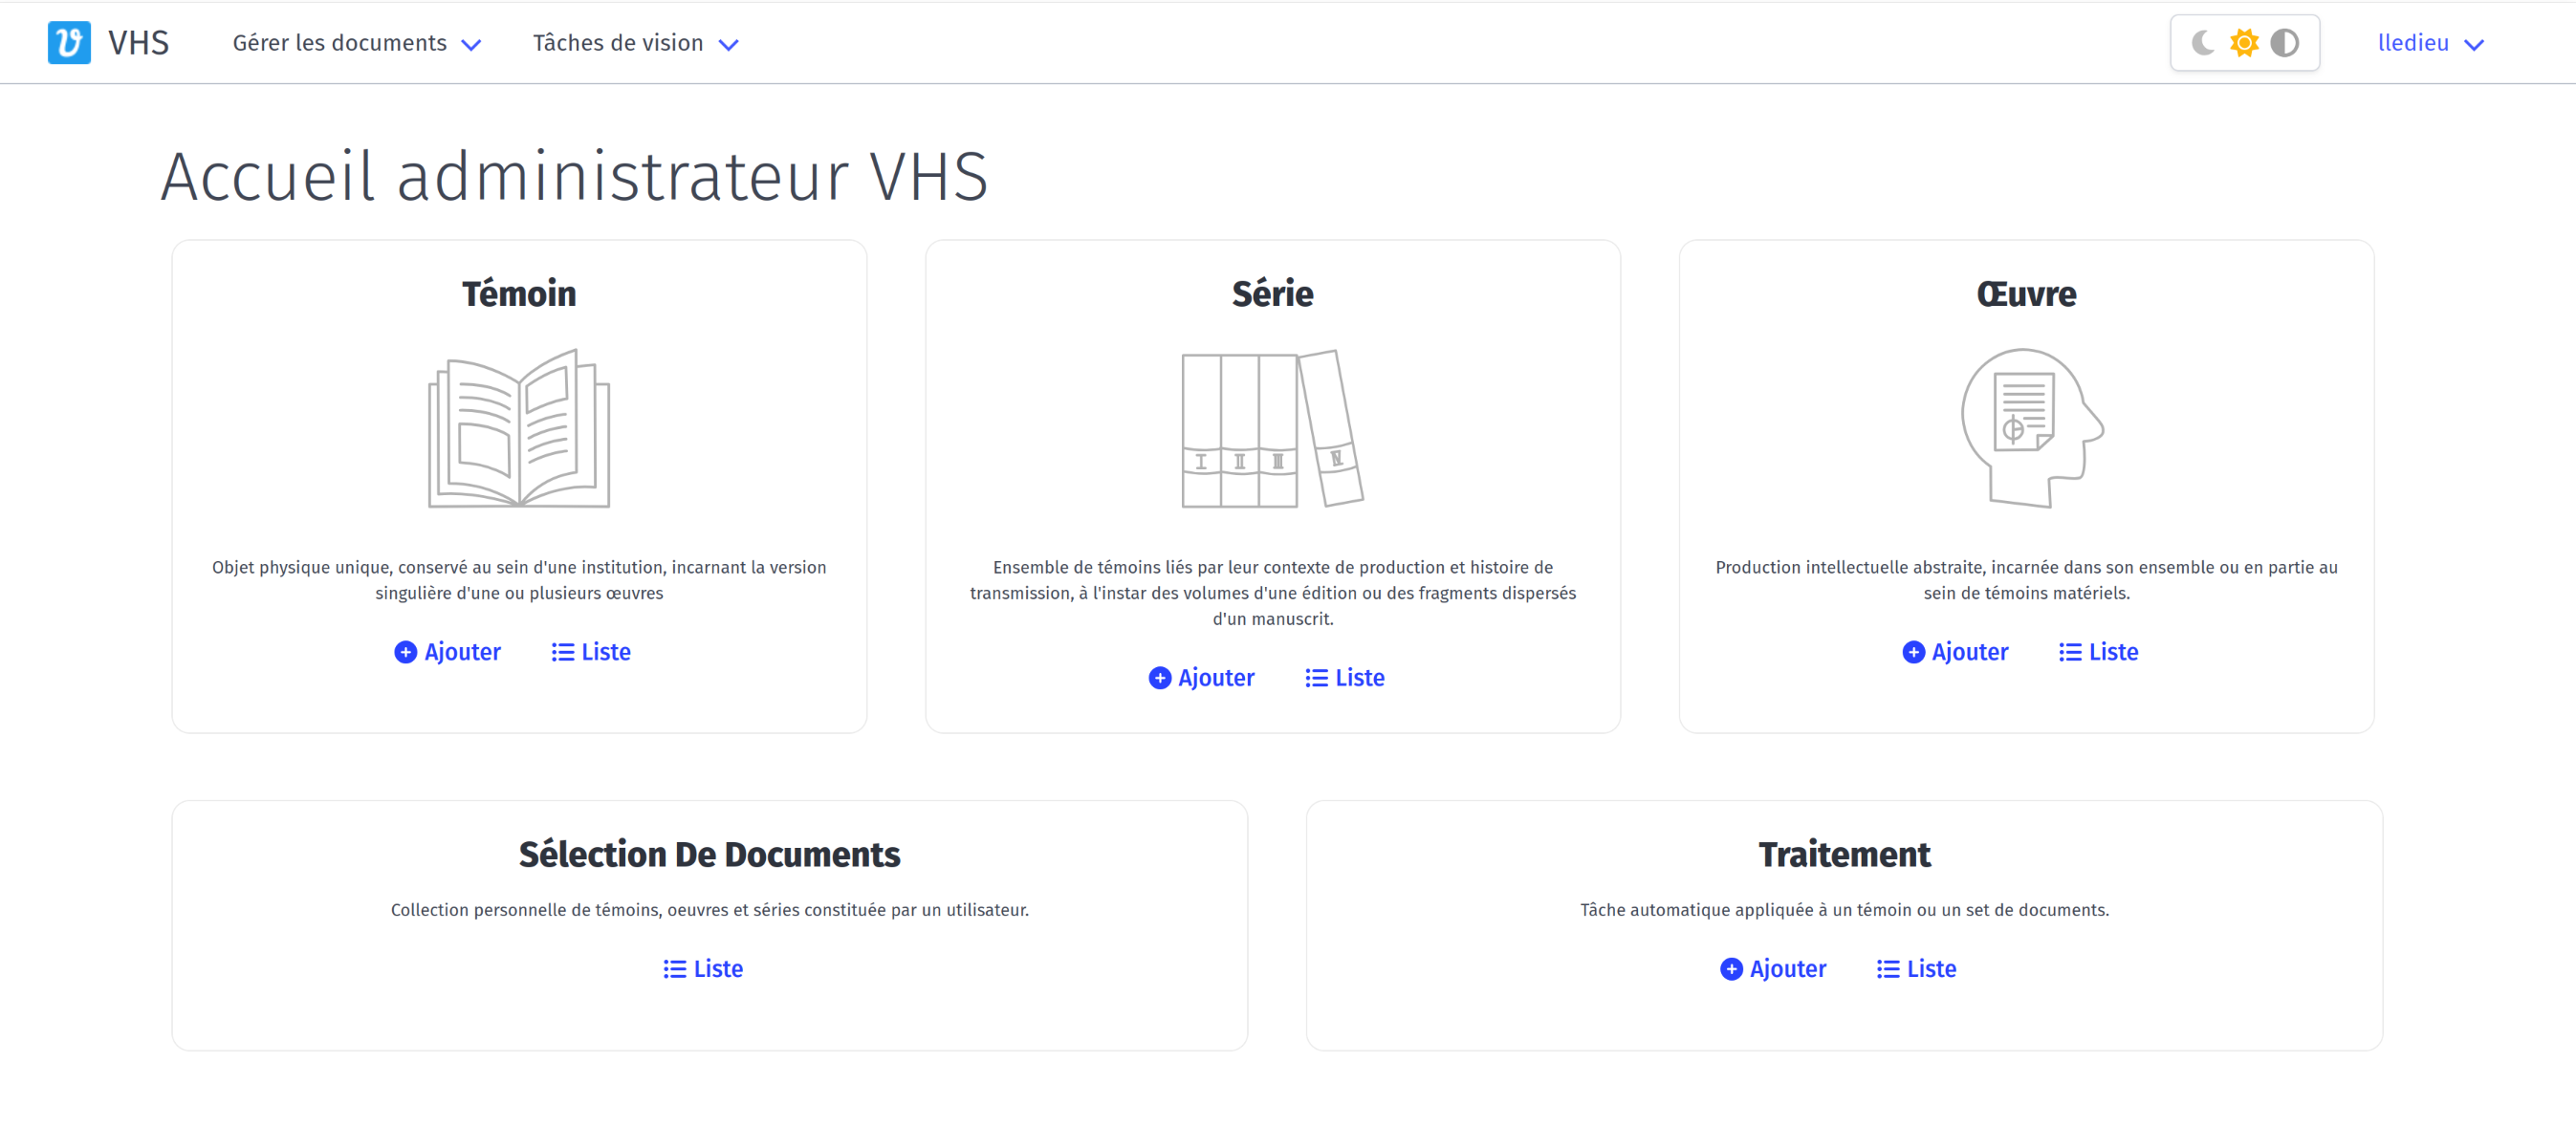
\includegraphics[width=\linewidth]{images/accueil_vhs.png}
	\end{subfigure}
	\caption{Interfaces administrateur EIDA et VHS}
	\label{fig:interface_accueil}
\end{figure}

Pour l'instant, ni \gls{vhs}, ni \gls{eida} ne possède d'interface publique. Les chercheurs utilisent actuellement l'interface administrateur, c'est-à-dire le \textit{back-office}. Ils possèdent chacun un compte avec un statut \og admin \fg tandis que les ingénieurs en charge du développement et de la gestion de l'application sont en mode \og super-admin \fg. L'avantage de ces interfaces est qu'il n'est pas nécessaire de savoir coder ou faire des requêtes \gls{sql}.

Un \textit{User's guide} détaillant les différentes options a été rédigé. Nous nous concentrerons sur les principales fonctionnalités.




\subsection{La constitution du corpus : gestion des sources numérisées}

Avant d'effectuer des traitements automatiques, l'application AIKON permet de constituer un corpus, le gérer et le partager. 

Pour ajouter la numérisation d'un document comme un manuscrit par exemple, il faut ajouter un nouveau  \textit{witness}. Il est possible de renseigner énormément de métadonnées pour le décrire comme sa cote, son lieu de conservation ou son type de pagination par exemple. Pour certaines catégories, comme c'est le cas avec le lieu de conservation, si celui de notre document n'est pas déjà disponible dans la base de données, nous devons le créer. Il pourra alors être réutilisé par les autres utilisateurs par la suite. En ce qui concerne le format de la numérisation, AIKON accepte les pdf, les manifestes \gls{iiif} ainsi que les images en format jpg ou png. 

Une fois le \textit{witness} ajouté à la base de données, les autres chercheurs inscrits sur la plateforme pourront accéder à lui et aux résultats des différents traitements qui lui seront appliqués. Un formulaire est d'ailleurs disponible pour affiner ses recherches.

\begin{figure}[H]
	\centering
	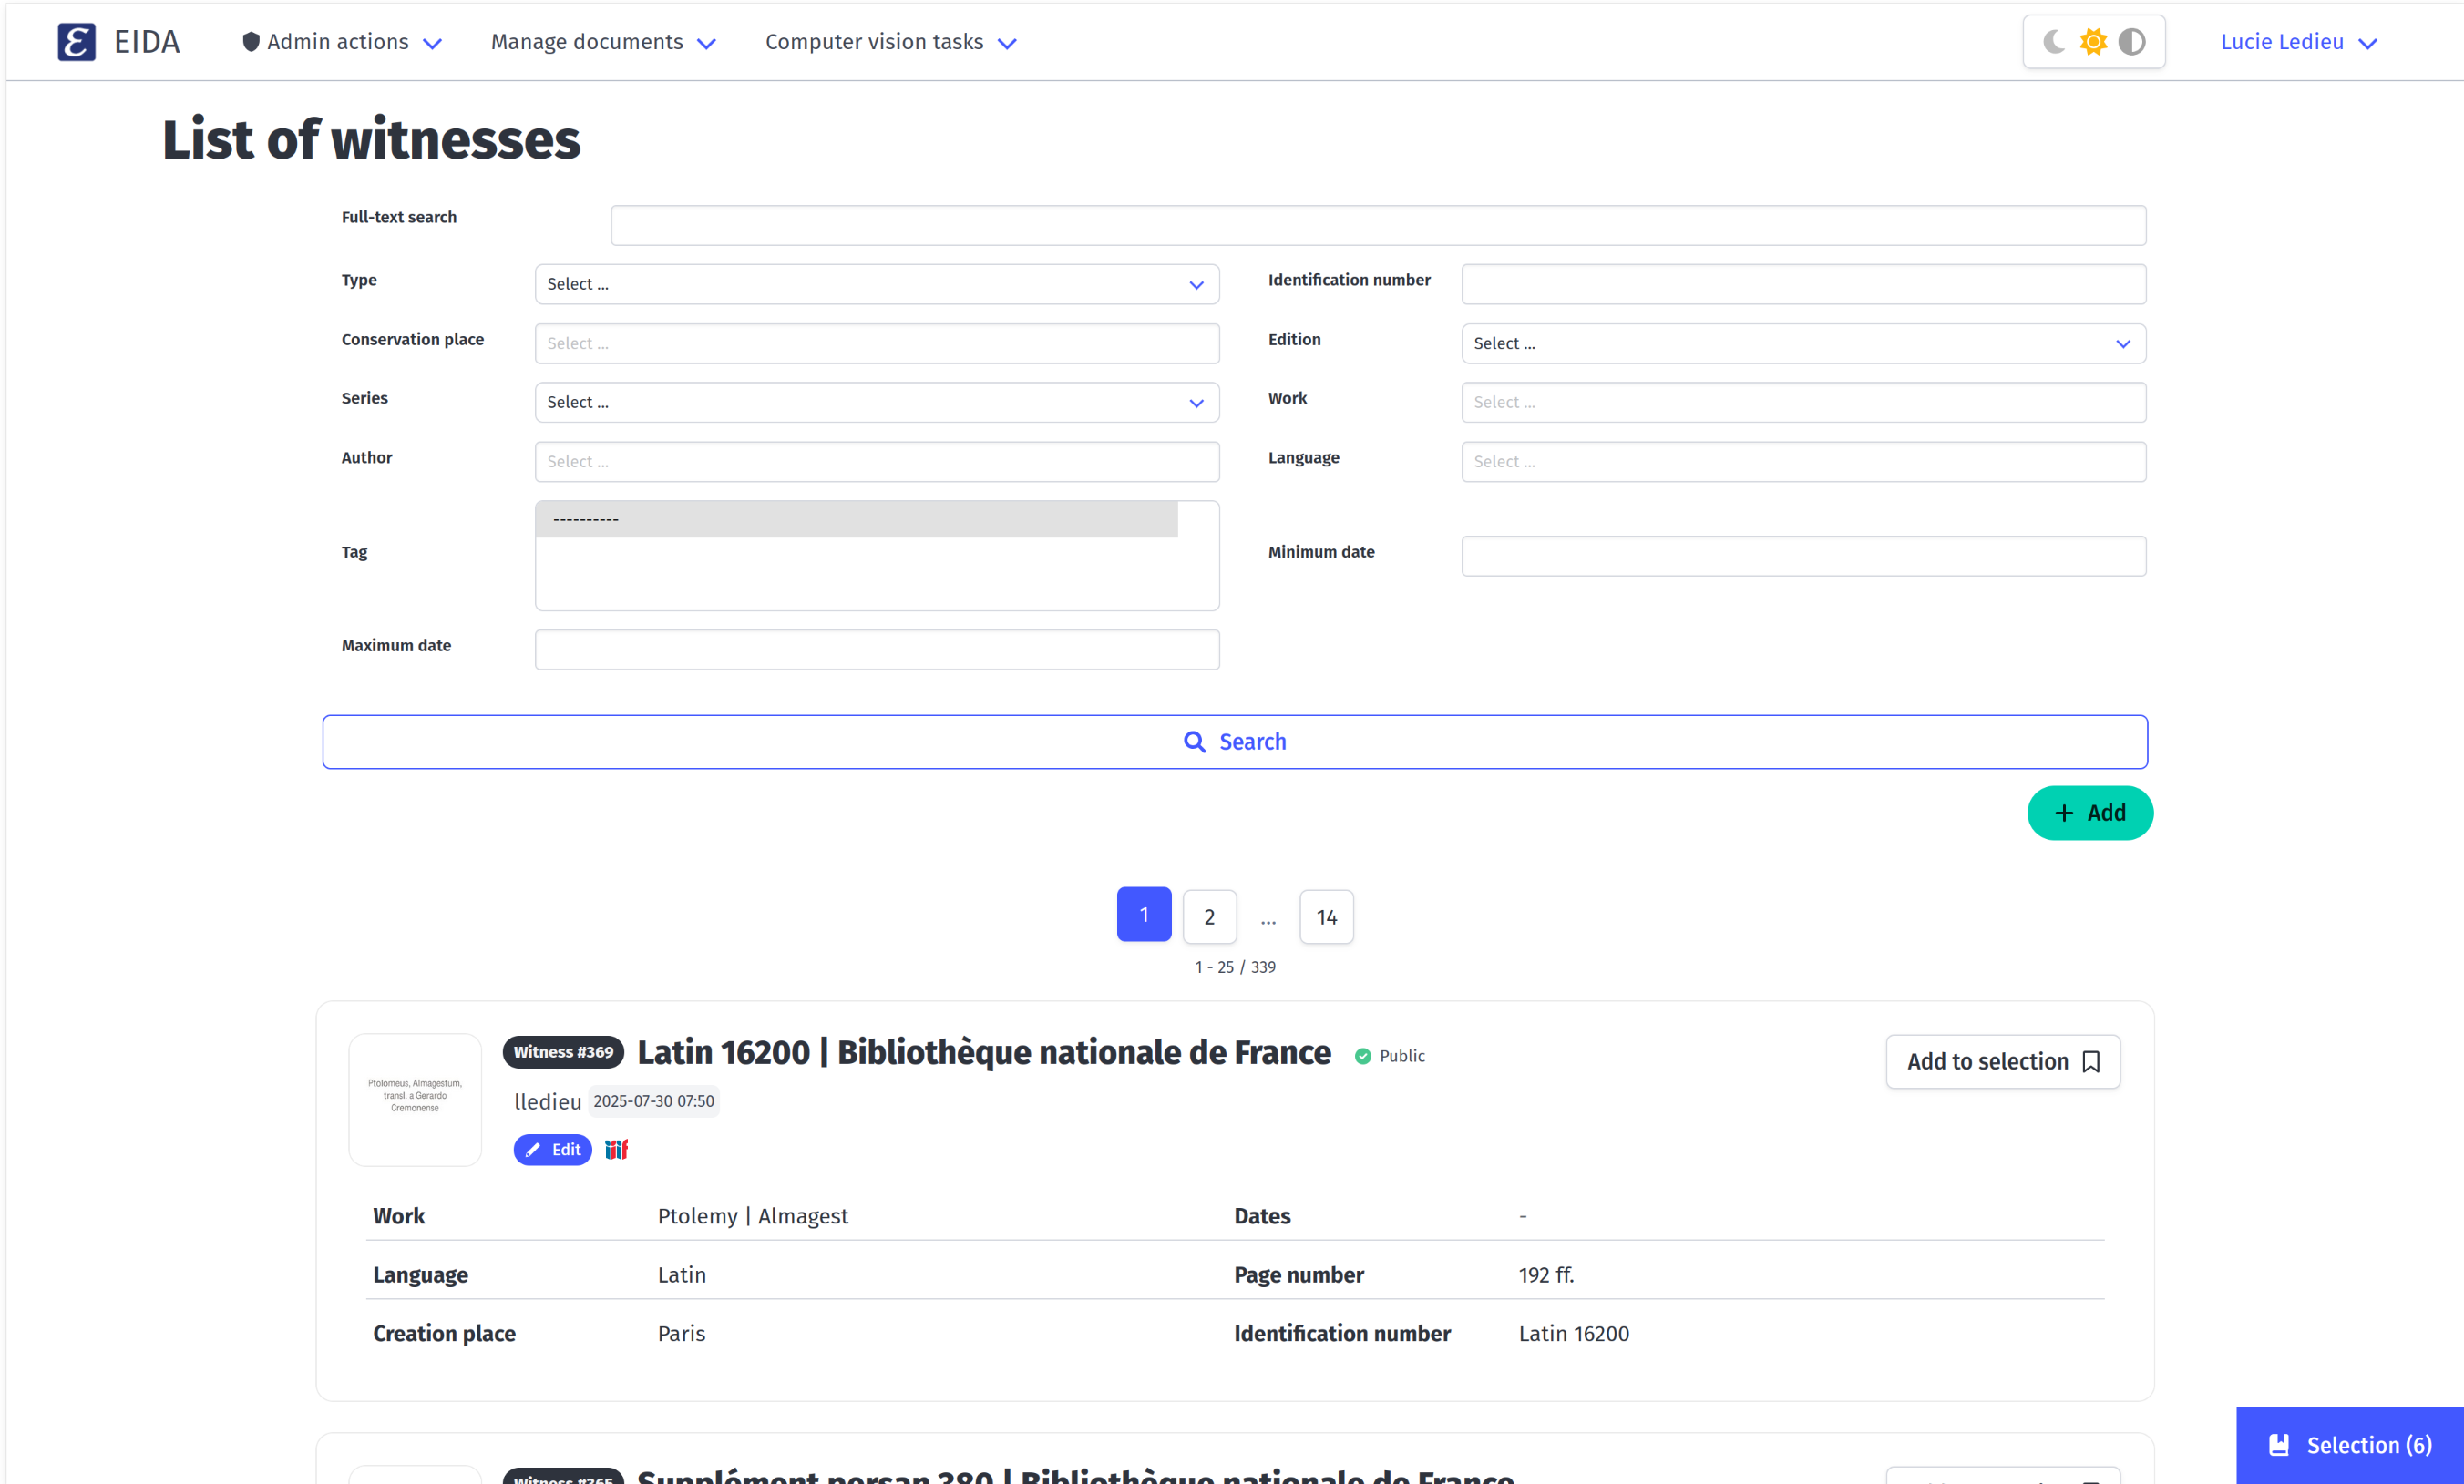
\includegraphics[width=0.8\textwidth]{images/list_witnesses.png}
	\caption{Capture d'écran de l'interface de consultation des différents \textit{witnesses} sur \gls{eida}}
	\label{fig:apercu_witnesses}
\end{figure}

Les différents \textit{witnesses} peuvent être organisés en sous-ensembles cohérents. Par exemple, nous pouvons réunir tous les volumes d'une même édition disponibles dans différentes institutions. Il est d'ailleurs aussi possible de réunir plusieurs \textit{witnesses} en un \textit{work} quand il s'agit de la même œuvre.

Pour créer sa propre collection de \textit{witnesses}, nous avons la possibilité de créer des \textit{document sets} en cliquant sur \og Add to selection \fg. Cette fonctionnalité est utile notamment lorsque nous voulons lancer un traitement pour plusieurs \textit{witnesses} à la fois.

\subsection{L'extraction des regions}

AIKON propose une fonctionnalité permettant d'extraire des \textit{regions}. Dans le cas d'\gls{eida}, il s'agit des diagrammes. Cette action peut se faire de manière manuelle, notamment lors de l'entraînement de l'algorithme ou lorsque ce dernier fait une erreur. 

\subsubsection{L'annotation manuelle avec Mirador}

Pour annoter de manière manuelle les \textit{regions} d'un \textit{witness}, il faut se servir de Mirador\footcite{MiradorHome}, un outil \textit{open-source} d'annotation d'image. Afin d'y accéder, il faut se rendre sur la page d'un des \textit{witnesses} et choisir \og \textit{Manually annotate}\fg. Pour définir une \textit{region}, il faut l'encadrer en utilisant le carré ou le cercle mis à disposition dans la barre de fonctionnalité.

\begin{figure}[H]
	\centering
	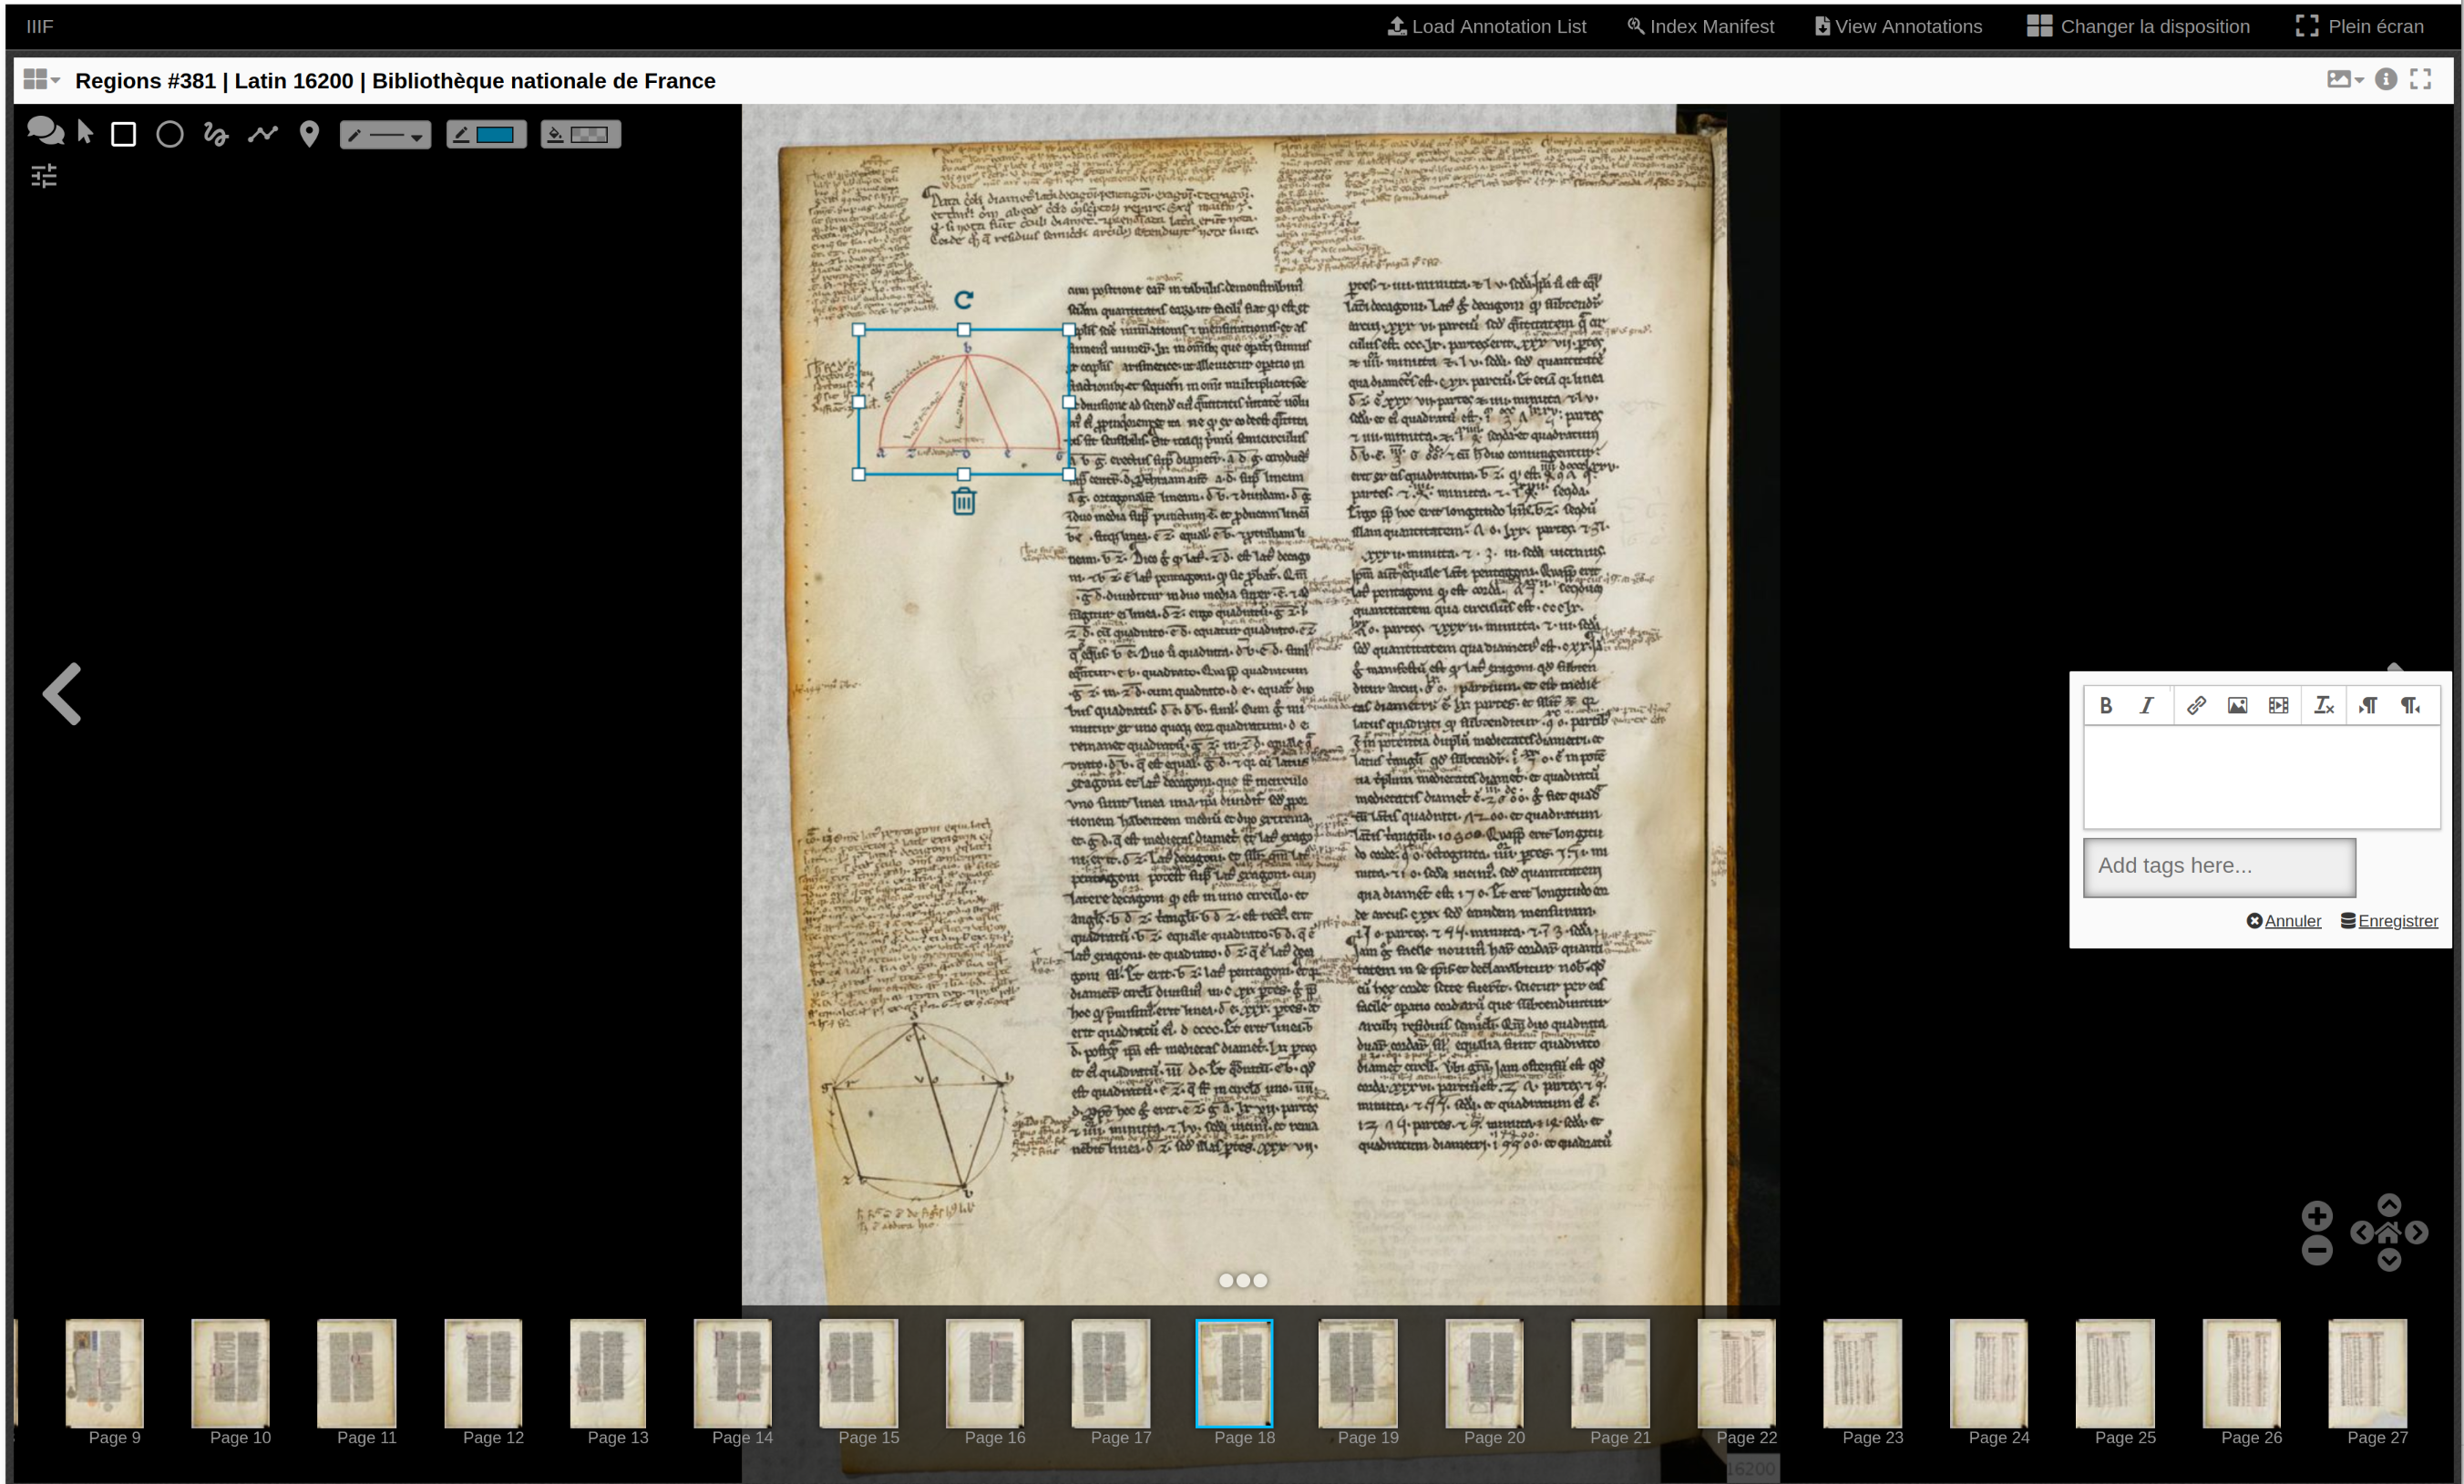
\includegraphics[width=0.8\textwidth]{images/capture_ecran_mirador.png}
	\caption{Aperçu de l'outil Mirador et de ses fonctionnalités}
	\label{fig:apercu_mirador}
\end{figure}


\subsubsection{L'extraction automatique des regions}

Annoter manuellement chaque \textit{region} est chronophage. Heureusement, il existe des algorithmes pour réaliser une extraction automatique de toutes les \textit{regions} d'un \textit{witness}. 
Pour faire cette opération, il faut se rendre sur la page d'un des \textit{witnesses} puis choisir \og textit{Automatic region extraction} \fg. Comme nous l'avons vu précédemment, il existe plusieurs algorithmes. Pour les diagrammes astronomiques, le plus approprié est \og \textit{Diagram extraction (YOLO model fine-tuned on historical diagrams)}\fg.


\begin{figure}[h]
	\centering
	\begin{subfigure}{0.48\linewidth}
		\centering
		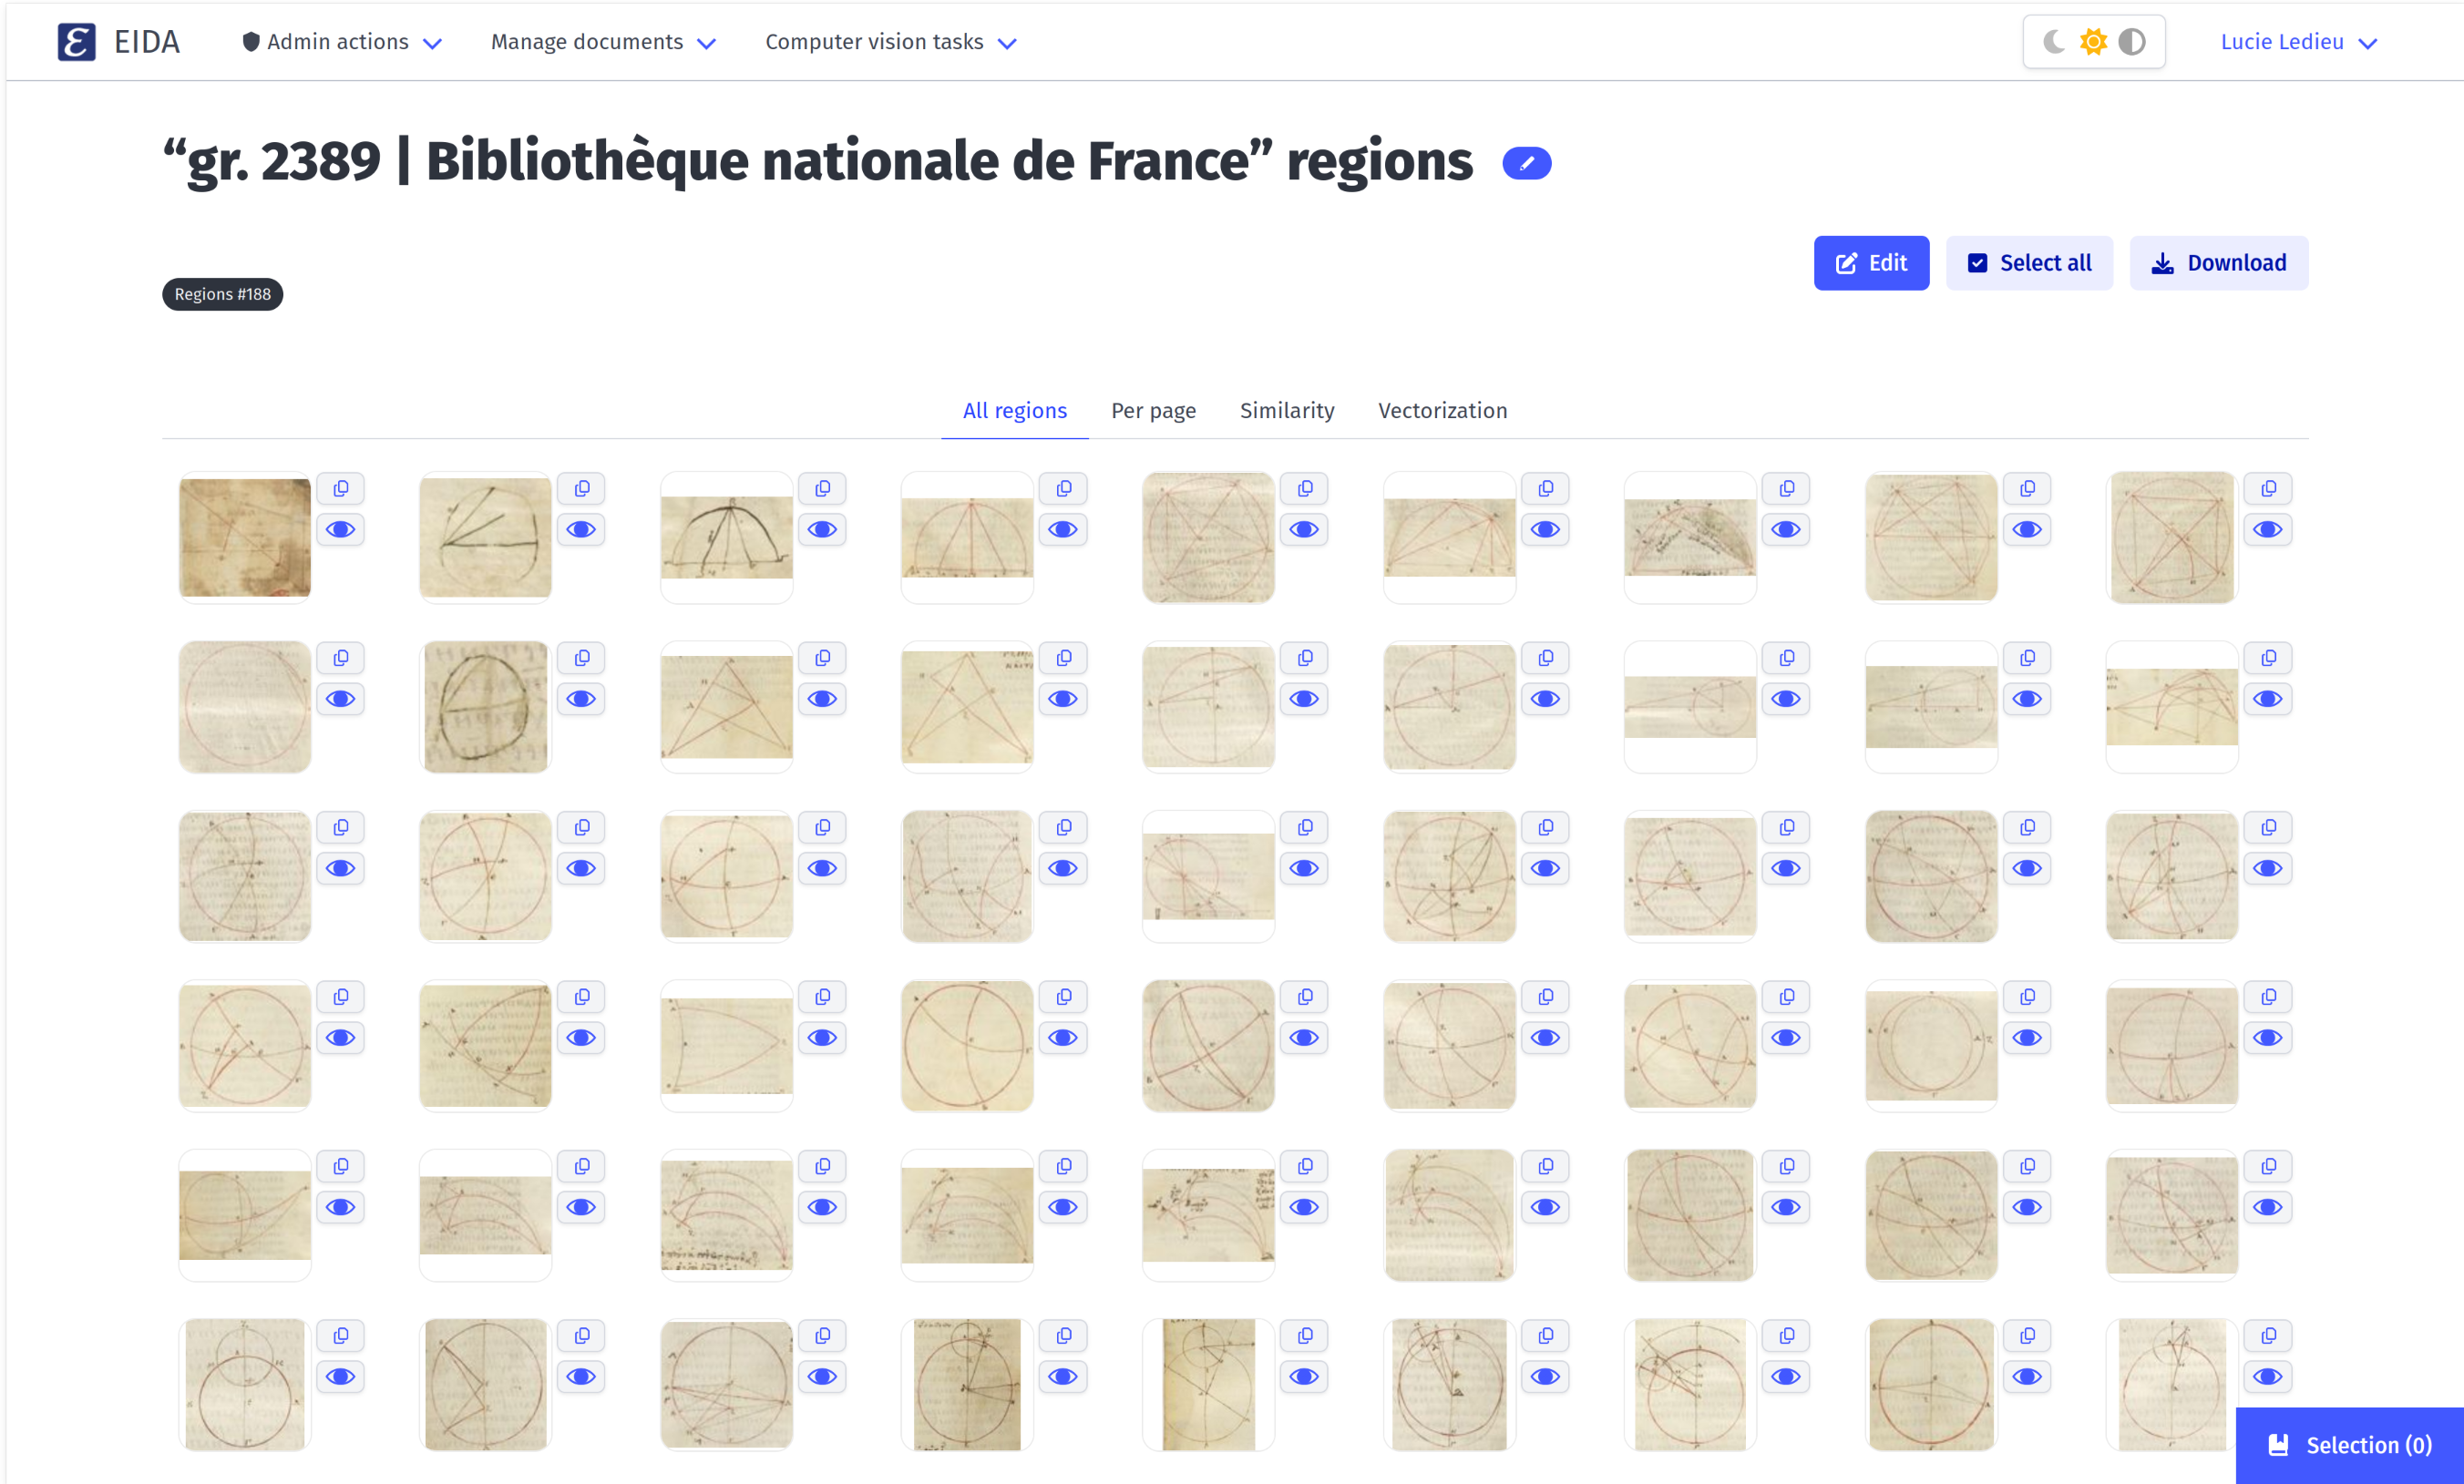
\includegraphics[width=\linewidth]{images/regions_par_witness.png}
	\end{subfigure}
	\hfill
	\begin{subfigure}{0.48\linewidth}
		\centering
		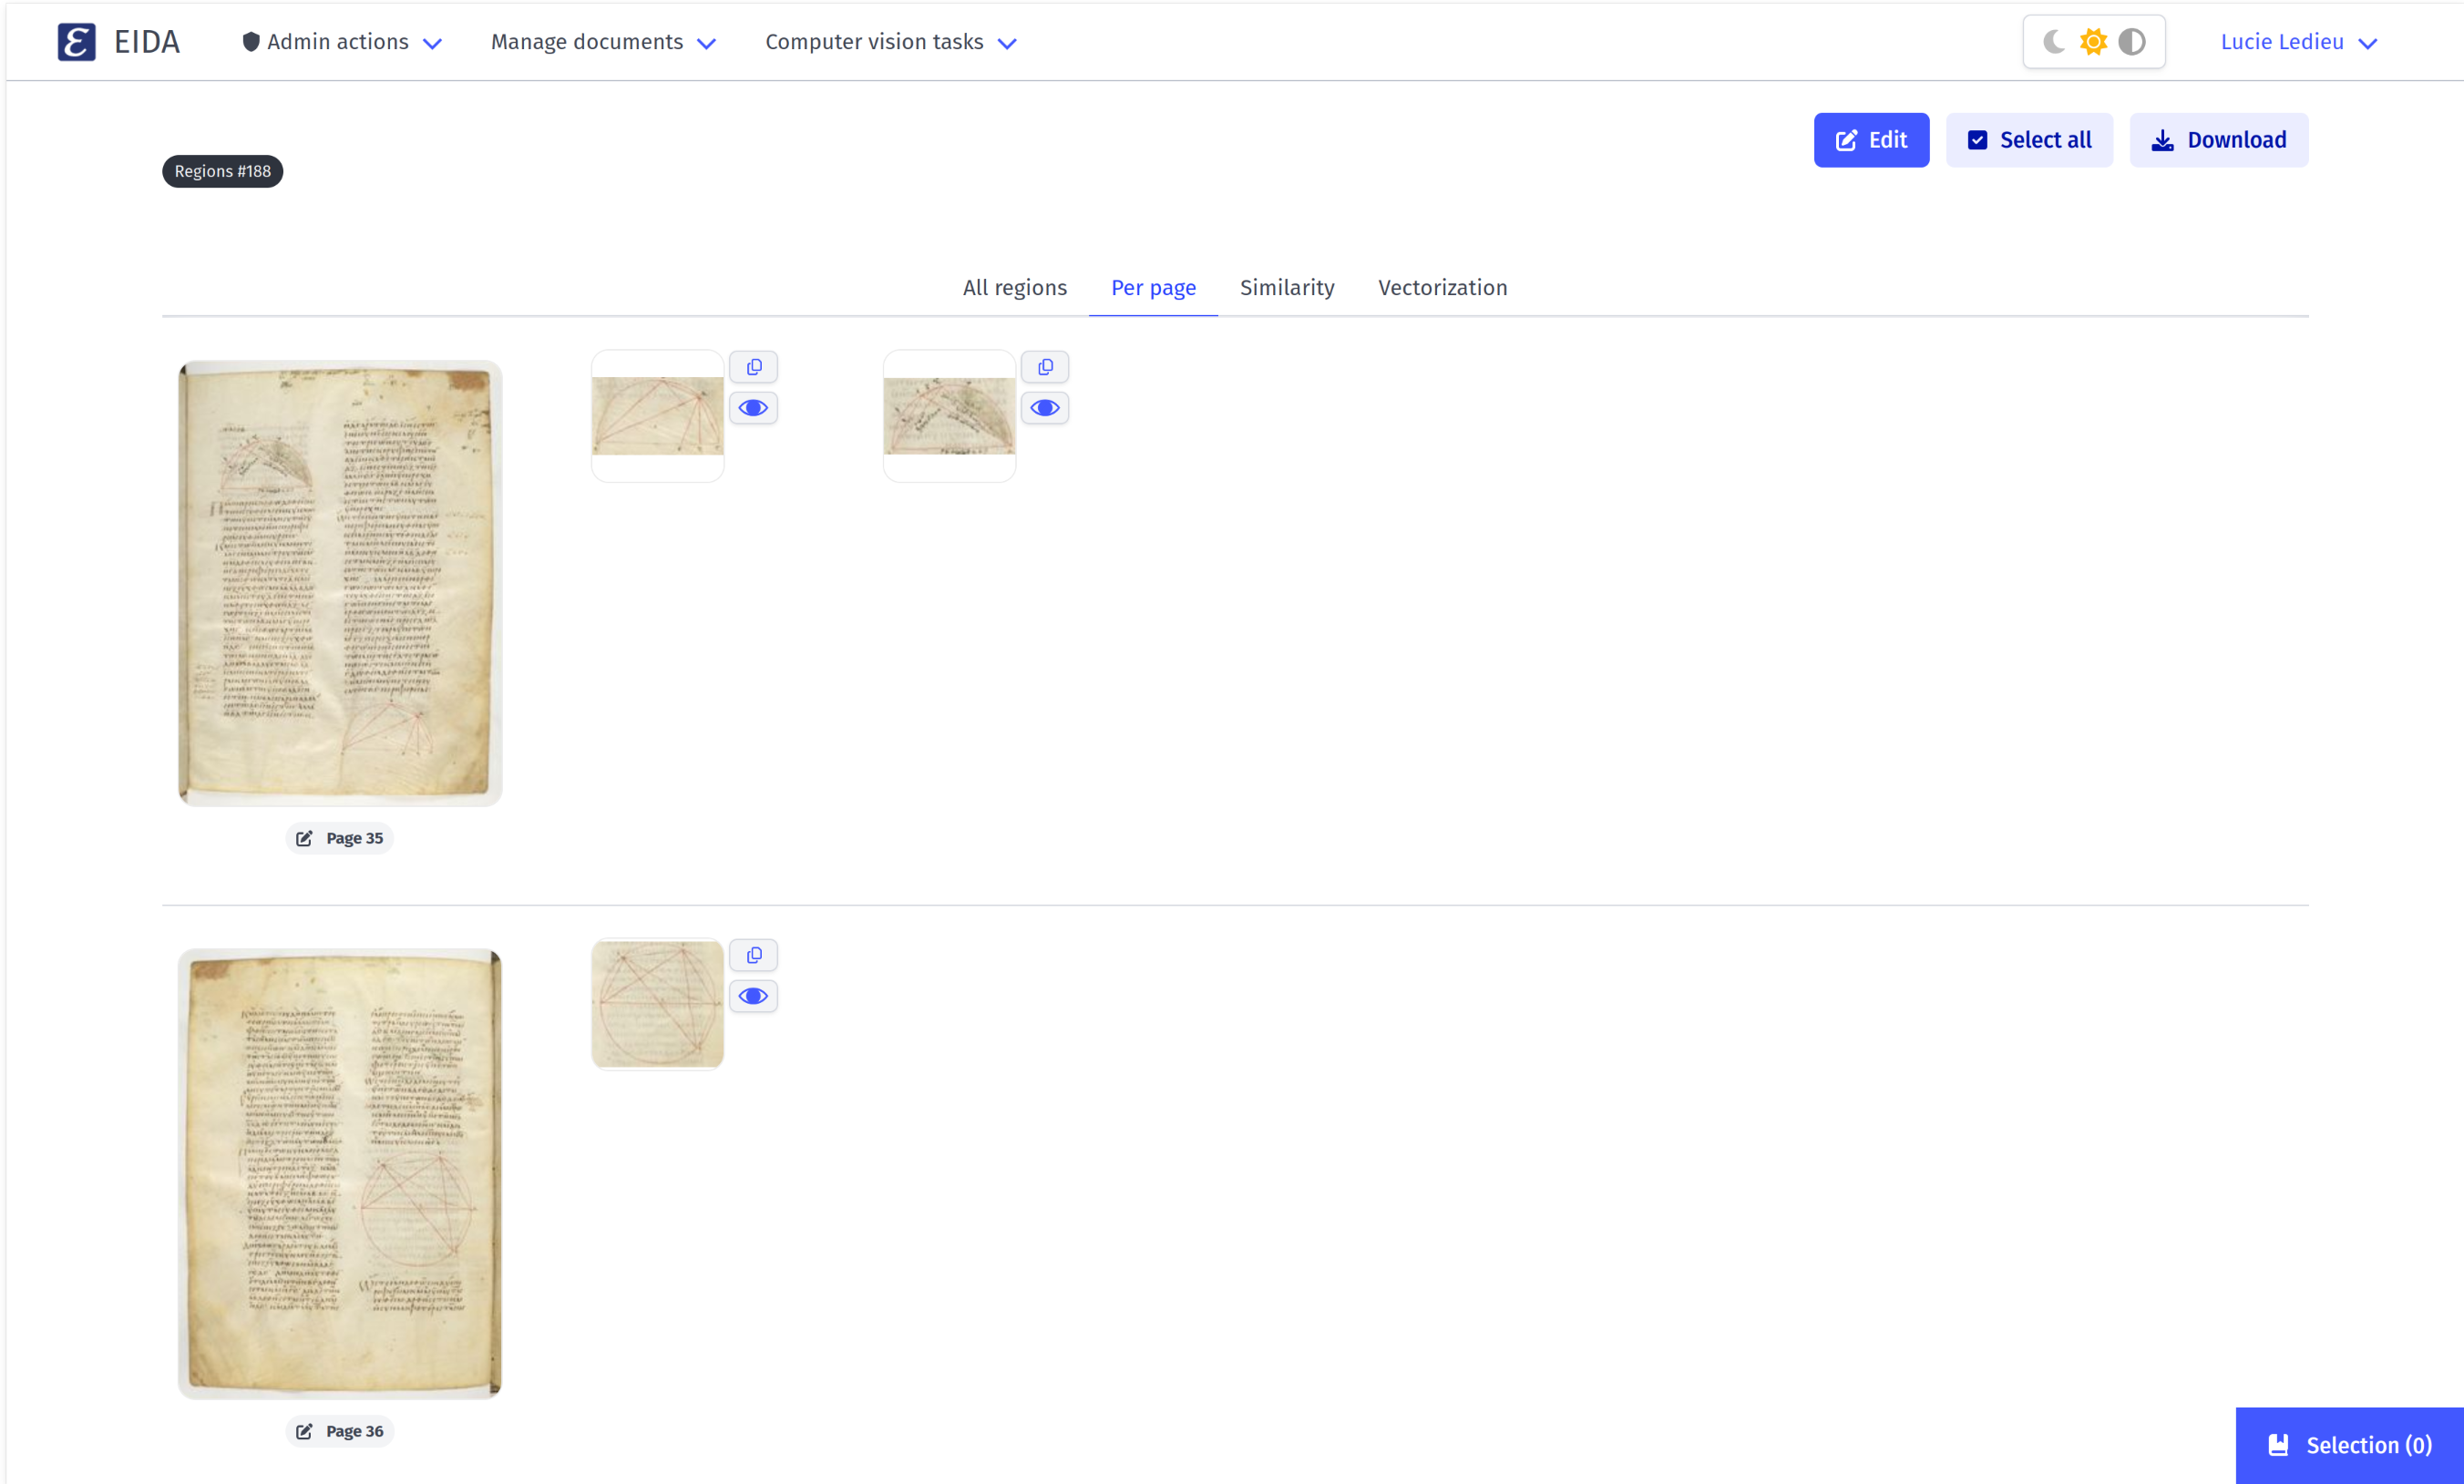
\includegraphics[width=\linewidth]{images/regions_par_page.png}
	\end{subfigure}
	\caption{\textit{Regions} extraites par \textit{witness} et par page}
	\label{fig:regions_extraction}
\end{figure}


Une fois le traitement terminé, nous pouvons visualiser les différents diagrammes extraits soit dans le \textit{witness} entier, soit page par page.

En cas d'erreur de l'algorithme, il est évidemment possible d'y remédier via Mirador.

\subsection{La constitution de correspondances entre les regions}

\subsubsection{La reconnaissance automatique et le calcul du score de similarités}

La plateforme AIKON propose une fonctionnalité de reconnaissance automatique de similarités couplée à la possibilité de calculer un score de similarité en chaque \textit{region} similaire. 

Pour commencer, il faut sélectionner les différents \textit{witnesses} à comparer dans un \textit{document set}. Ensuite, nous devons nous rendre dans l'onglet \og \textit{Computer vision tasks} \fg puis cliquer sur \og \textit{Add new treatment} \fg et choisir \og \textit{Compute similarity score} \fg dans \og \textit{Task type} \fg. Il est aussi possible de faire une extraction automatique de \textit{regions} dans plusieurs \textit{witnesses} au même endroit. Pour extraire des diagrammes, la meilleure solution est d'utiliser l'algorithme \textit{SegSwap} que nous avions cité précédemment. 

\begin{figure}[H]
	\centering
	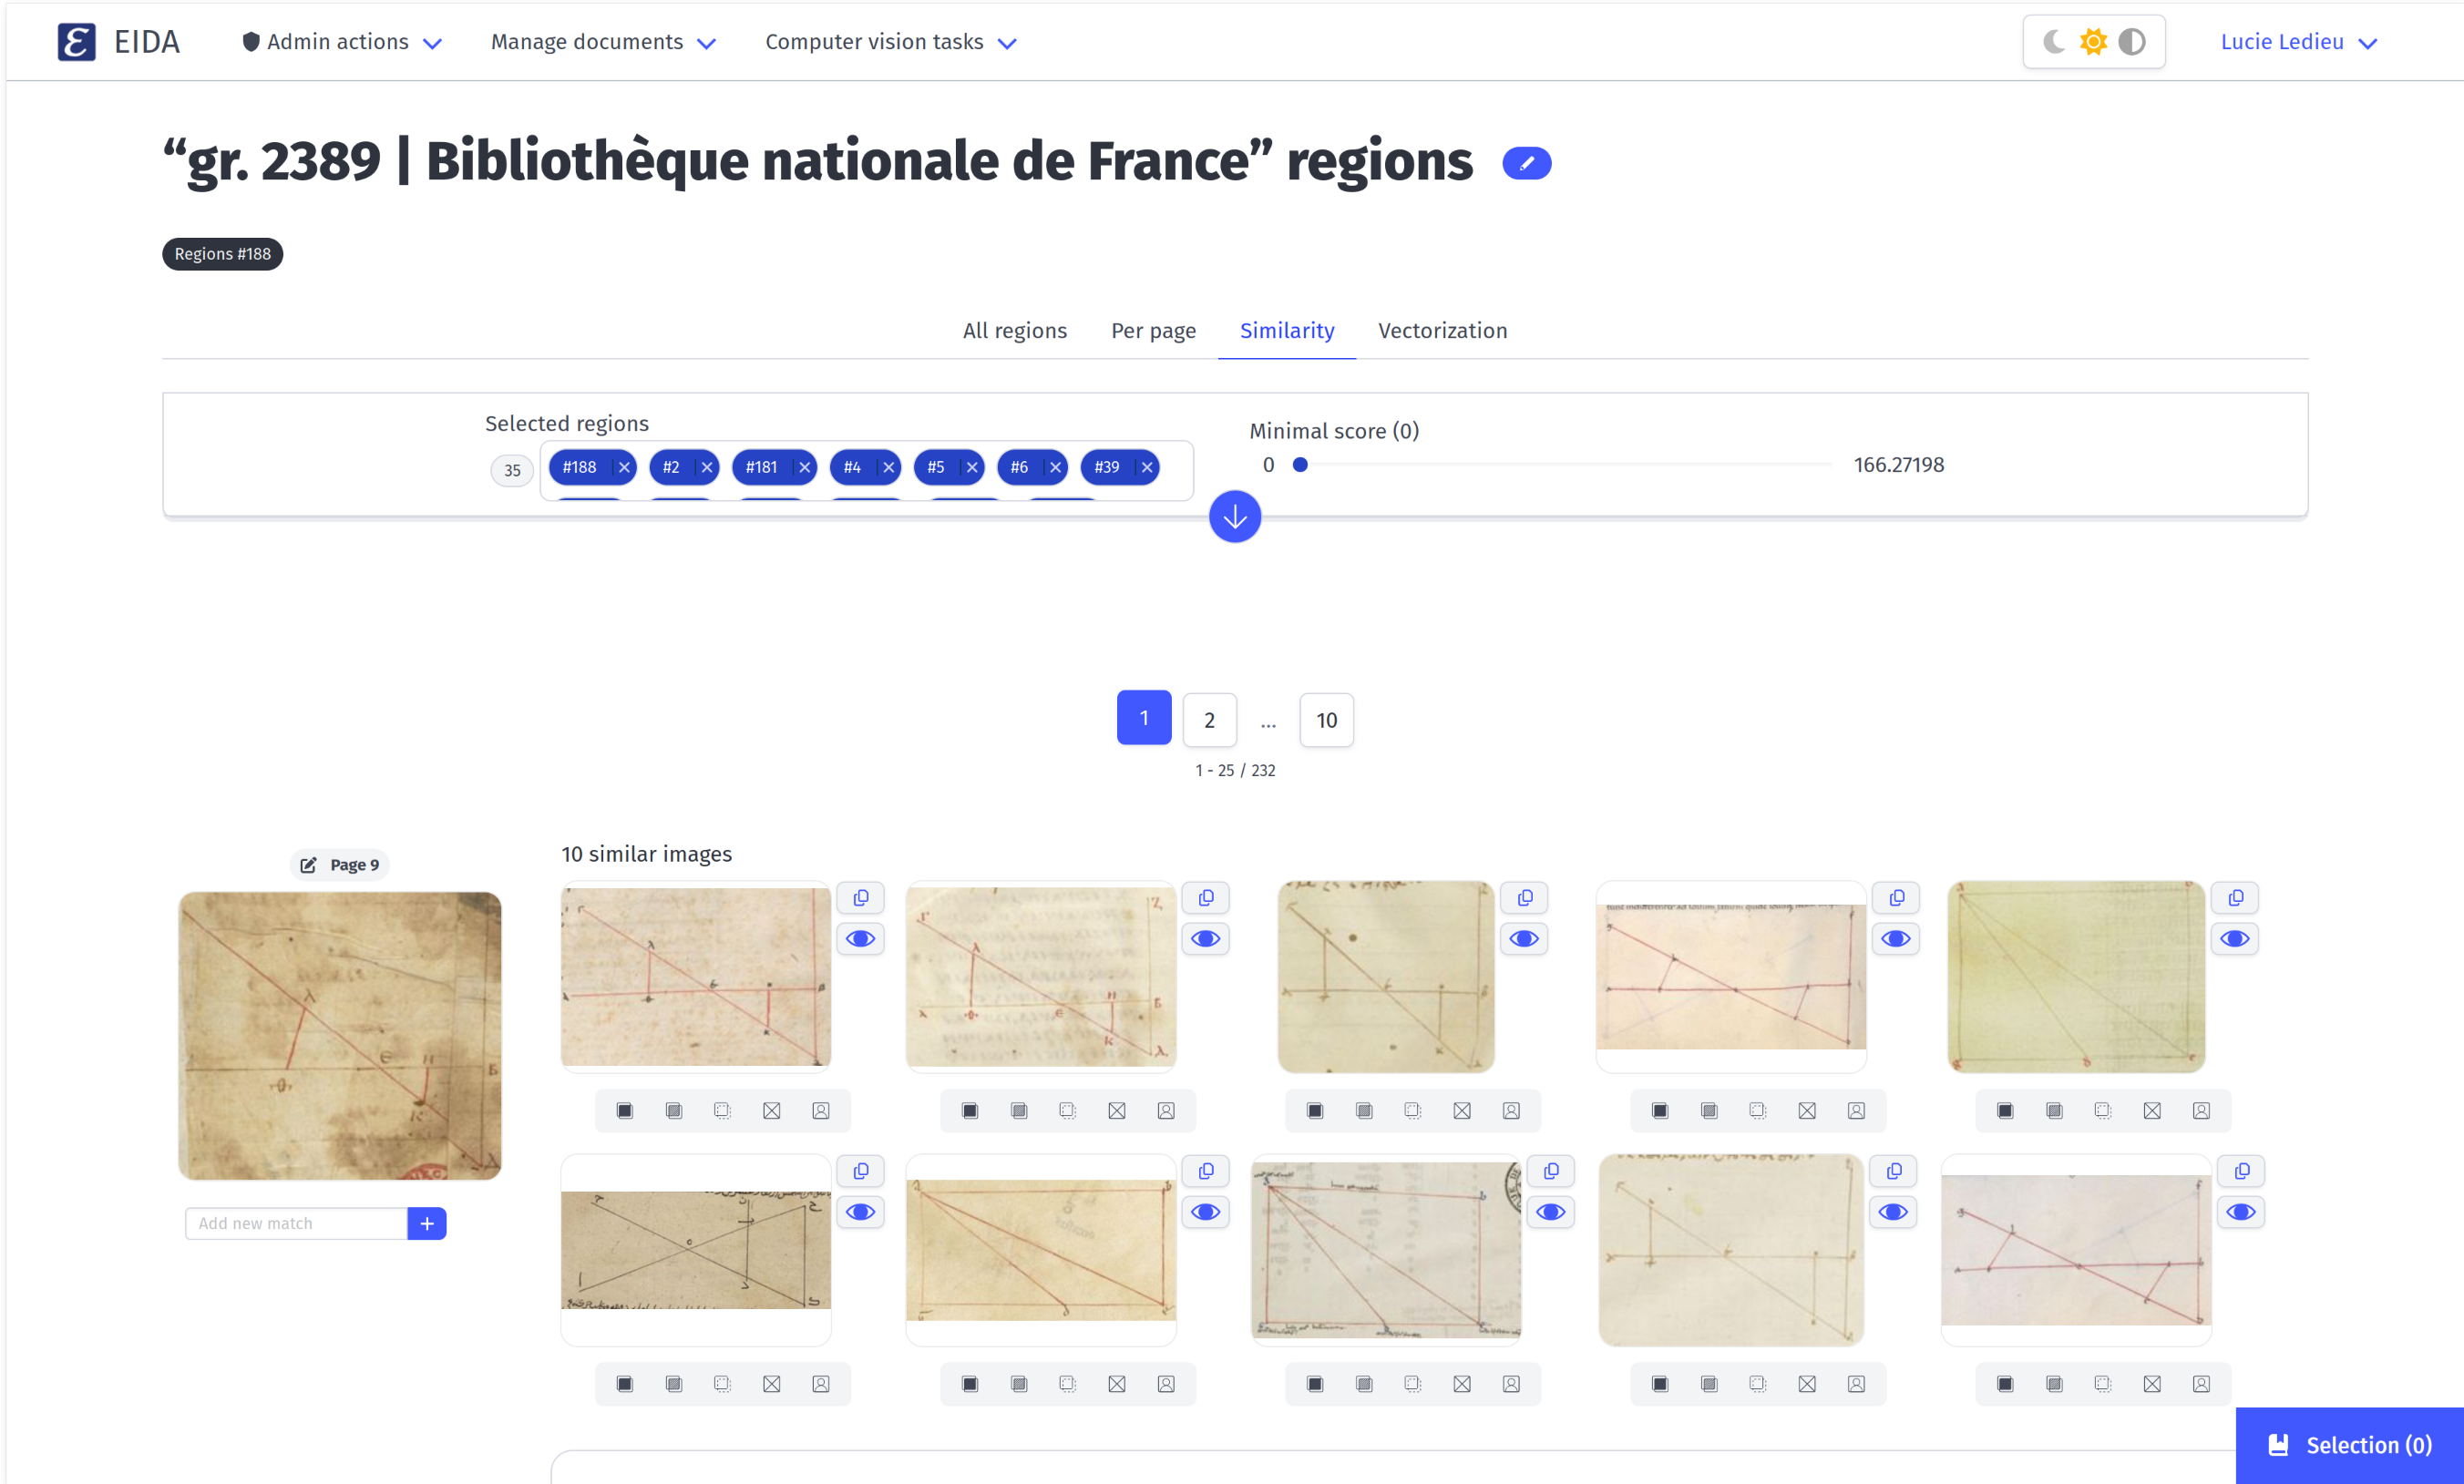
\includegraphics[width=0.8\textwidth]{images/similarities.png}
	\caption{Aperçu des différentes \textit{regions} similaires dans un \textit{witness}}
	\label{fig:apercu_similarites}
\end{figure}

Une fois le traitement réalisé, nous pouvons observer les résultats en retournant sur un des \textit{witnesses}. 
IL est possible de les filtrer grâce au formulaire en haut qui propose de choisir quels \textit{witnesses} nous voulons comparer. IL y a également un curseur pour choisir le score de similarité minimal.

\subsubsection{L'annotation des résultats}


Même si l'objectif final serait de créer des outils d'intelligence artificielle qui n'ont pas besoin d'être annotés au préalable, nous sommes à une étape du projet où il est encore nécessaire de le faire pour entraîner les algorithmes.

\begin{figure}[H]
	\centering
	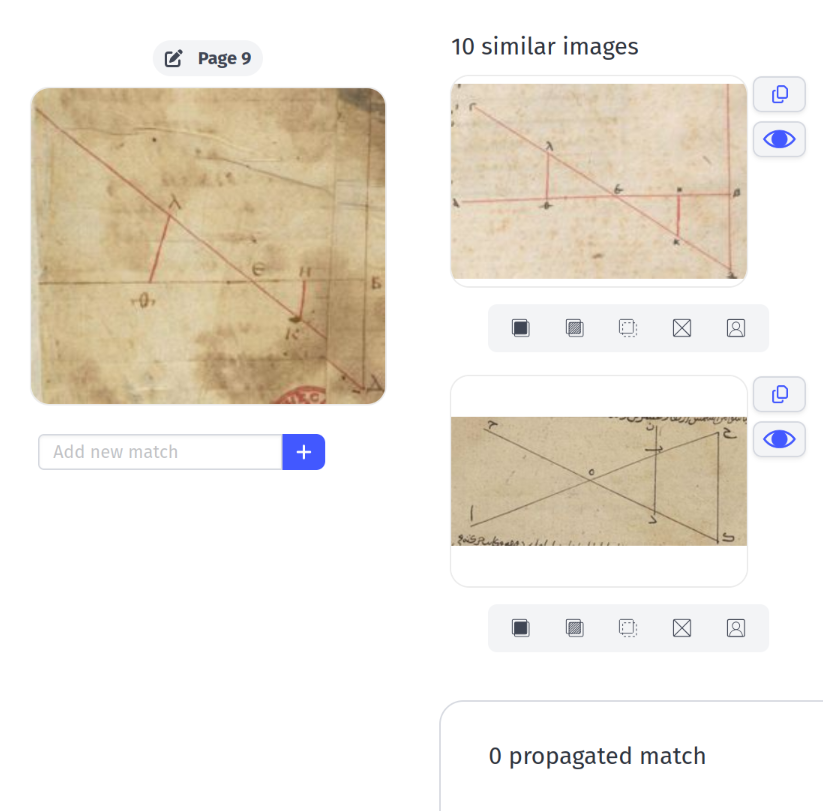
\includegraphics[width=0.8\textwidth]{images/annotation_similarities.png}
	\caption{Aperçu de l'interface d'annotation des similarités}
	\label{fig:annotations_similarites}
\end{figure}

Pour annoter les différentes \textit{regions}, il y a un petit panneau en dessous de chacune d'entre-elles avec plusieurs cases qui représentent le type d'annotation : 
\begin{enumerate}
	\item \textit{Exact match} : Les deux \textit{regions} sont parfaitement similaires.
	\item \textit{Partial match} : Les deux \textit{regions} sont un peu différentes.
	\item \textit{Semantic match} : Les deux \textit{regions} sont différentes physiquement mais d'un point de vue théorique elles représentent un même concept ou signification.
	\item \textit{No match} : les deux \textit{regions} ne sont pas du tout similaires.
\end{enumerate} 


En ce qui concerne le projet \gls{eida}, l'objectif final serait de développer une interface publique sur le même modèle que celle du projet \gls{dishas}.

\begin{figure}[H]
	\centering
	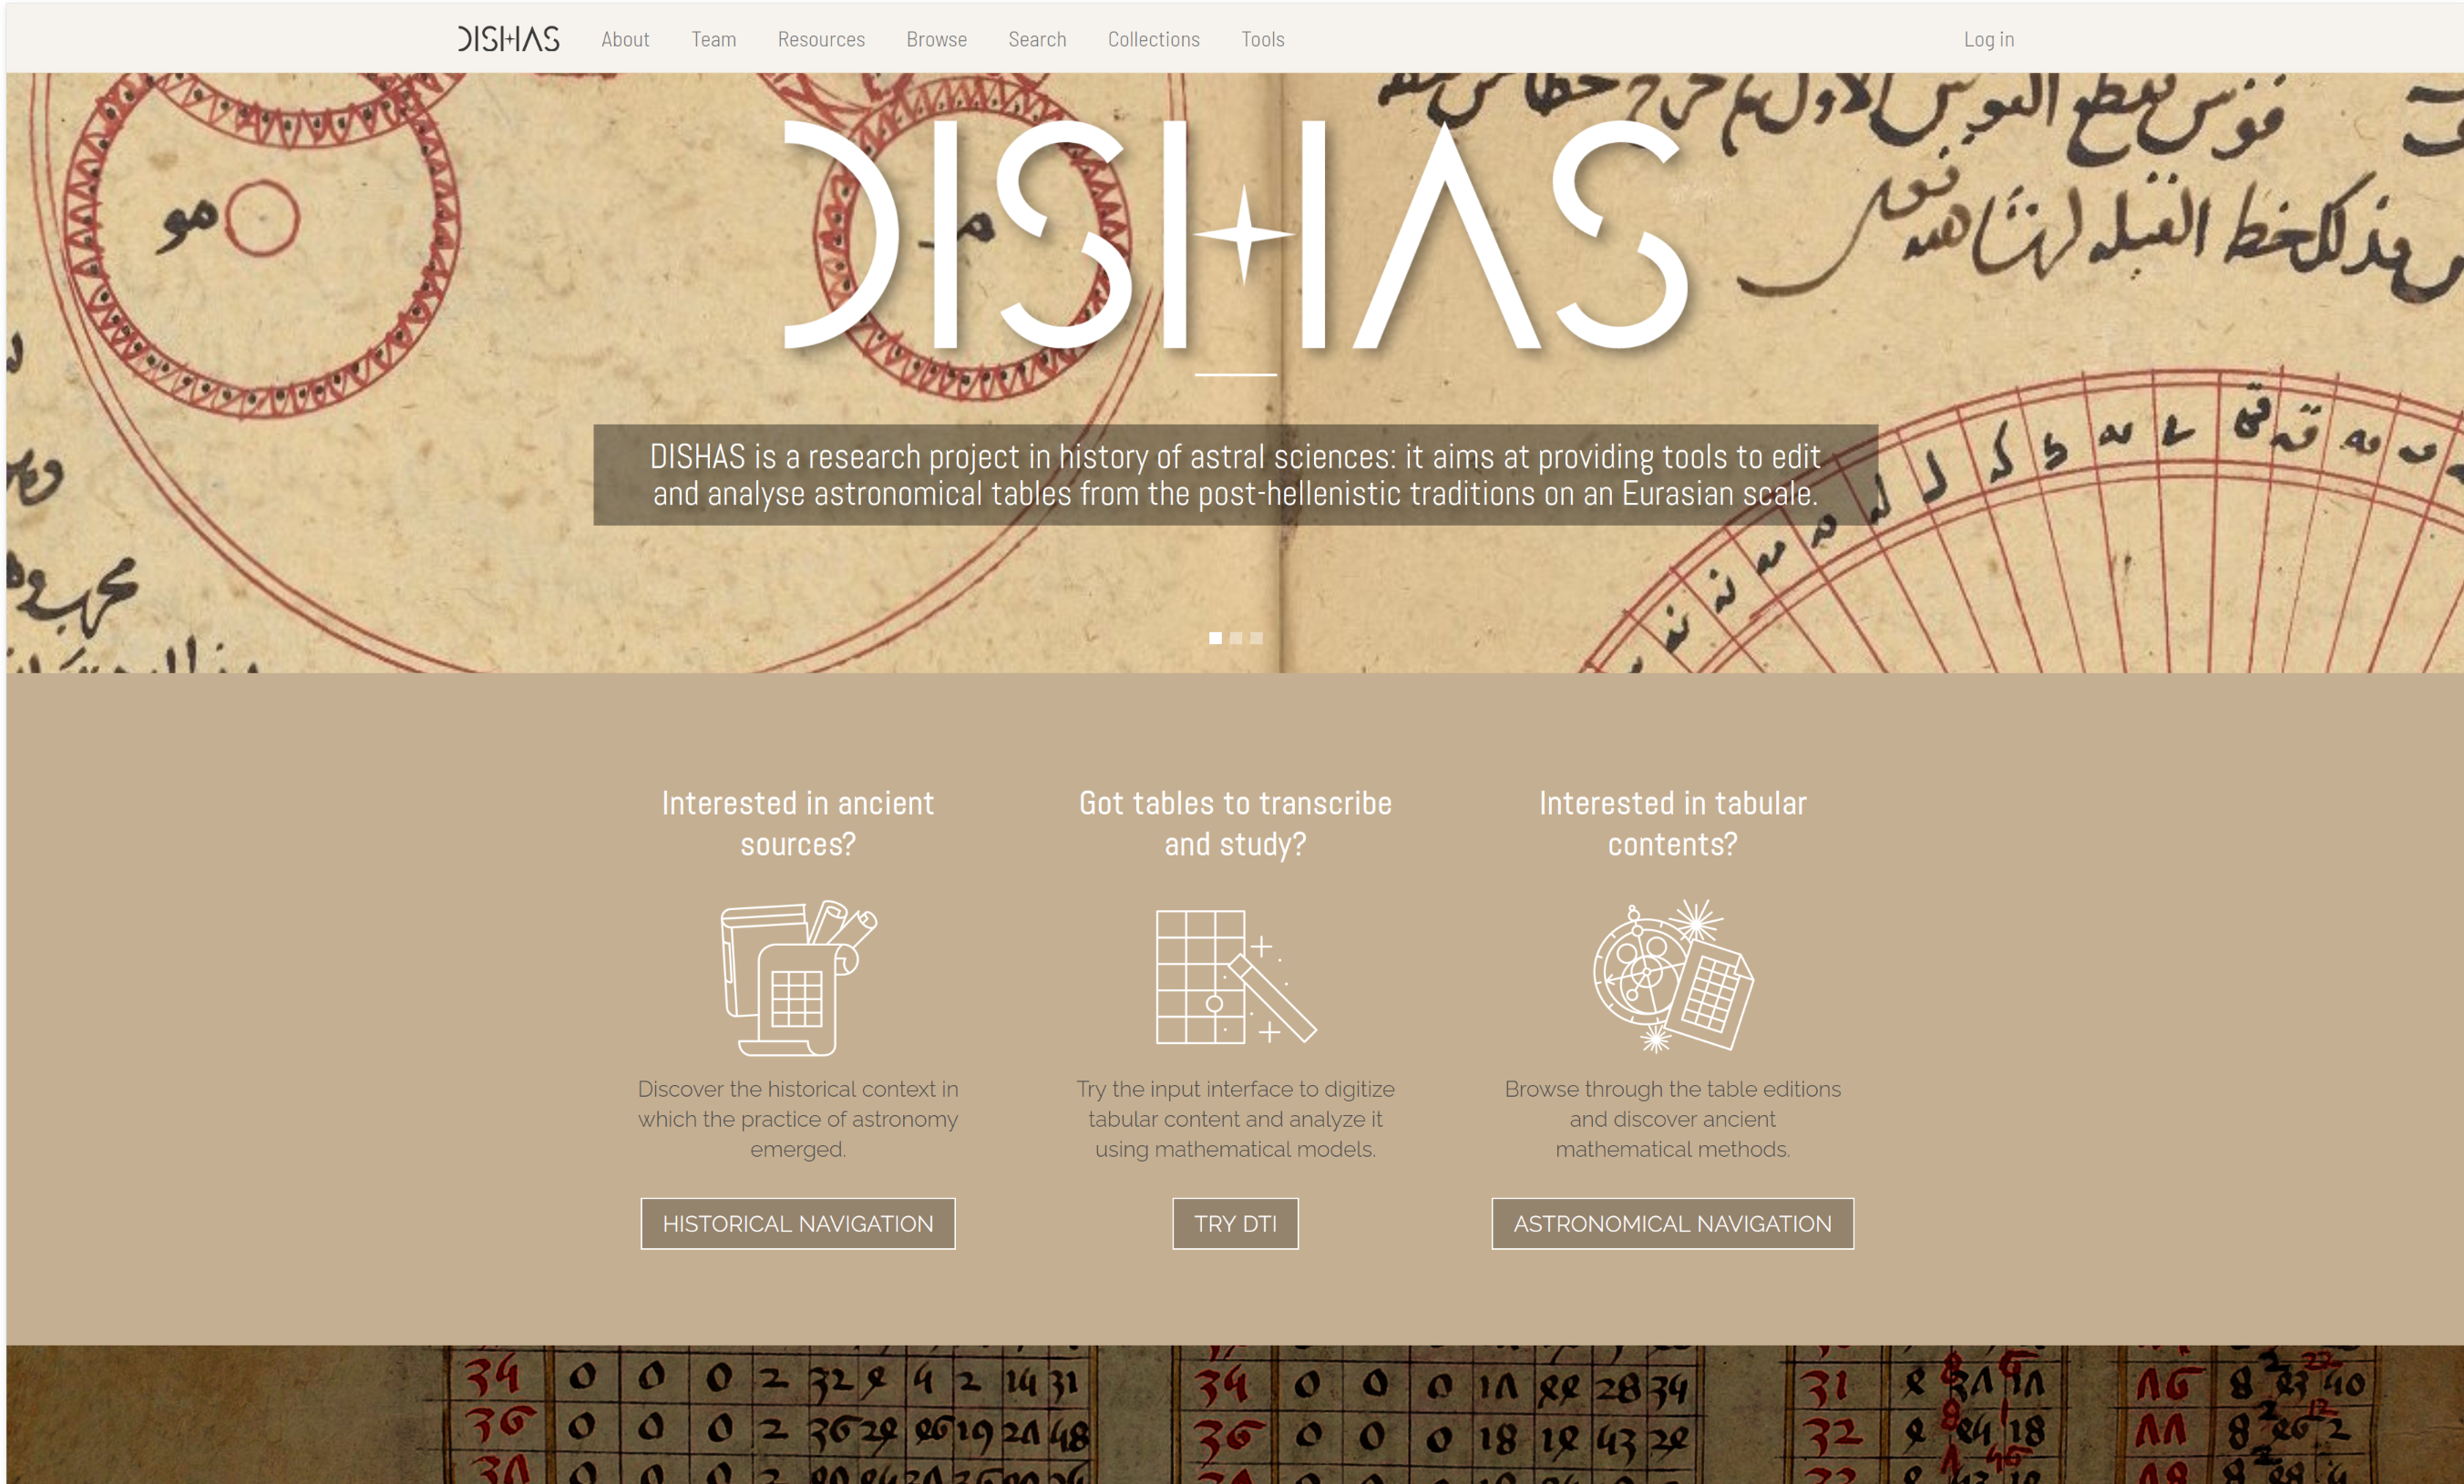
\includegraphics[width=1\textwidth]{images/dishas.png}
	\caption{Capture d'écran de l'interface publique de \gls{dishas}}
	\label{fig:dishas-interface}
\end{figure}

L'objectif principal d'une interface publique ou \textit{front-office} est de mettre à disposition des utilisateurs les différents outils développés au cours du projet ainsi que les résultats obtenus. Lors de sa création, le dialogue avec les chercheurs est primordial. En effet, il doit y avoir un \og fil conducteur \fg suivant les différentes hypothèses scientifiques ayant orienté leur réflexion dans la navigation entre les différentes pages. Les données doivent être contextualisées dans leur corpus ainsi que dans le projet en général\footcite{albouyMediationDonneesRecherche2019}.Dans ce contexte, il est essentiel de réaliser des visualisations afin de les rendre accessible, de mieux les comprendre et de les explorer de manière interactive. 
	
	\clearemptydoublepage
	
	\chapter{Vers la nécessité d'interfaces d'exploration}
	\section{Masse de données et limites de l'exploration manuelle}
	\include{templates/section}
	
	\section{De la correction d'annotations à l'interprétation scientifique}
	\include{templates/section}
	
	\section{Questions de recherche et besoins d'exploration du corpus}
	\include{templates/section}
	
	\clearemptydoublepage
	
	
	\part{Méthodologie de conception des visualisations exploratoires}
	\chapter{La visualisation en histoire}
	\section{Evolution des représentations visuelles en histoire}
	\include{templates/section}
	
	\section{Visualisations de réseaux et étude des disséminations}
	\include{templates/section}
	
	\section{Enjeux critiques de la médiation numérique des données historiques}
	\include{templates/section}
	
	\clearemptydoublepage
	
	\chapter{Formalisation des besoins et contraintes de conception}
	\section{Analyse des pratiques et questions des chercheurs EIDA}
	\include{templates/section}
	
	\section{Cahier des charges : objectifs scientifiques et contraintes techniques}
	\include{templates/section}
	
	\section{Choix méthodologiques : network graph et alignement des sources (bipartite)}
	\include{templates/section}
	
	\clearemptydoublepage
	
	\chapter{Processus itératif de développement}
	\section{Prototypage et tests de faisabilité technique}
	\include{templates/section}
	
	\section{Mise en oeuvre concrète : choix techniques et difficultés rencontrées}
	\include{templates/section}
	
	\section{Intégration des retours utilisateurs et ajustements}
	\include{templates/section}
	
	\clearemptydoublepage
	
	\part{Evaluation critique et perspectives d'intégration}
	\chapter{Analyse des visualisations produites}
	\section{Visualisation bipartite : révéler les réorganisations du contenu intellectuel}
	\include{templates/section}
	
	\section{Network graph : explorer les chaînes de transmissions}
	\include{templates/section}
	
	\section{Adéquation aux objectifs d'exploration scientifique}
	\include{templates/section}
	
	\clearemptydoublepage
	
	\chapter{Validation et limites méthodologiques}
	\section{Critères d'évaluation de l'efficacité exploratoire}
	\include{templates/section}
	
	\section{Retour d'expérience par les chercheurs}
	\include{templates/section}
	
	\section{Limites liées aux données et biais d'interprétation}
	\include{templates/section}
	
	\clearemptydoublepage
	
	\chapter{Perspectives d'évolution et généralisation}
	\section{Intégration dynamique à la plateforme AIKON}
	\include{templates/section}
	
	\section{Transférabilité vers d'autres corpus et projets}
	\include{templates/section}
	
	\section{Implications pour l'évolution des pratiques en humanités numériques}
	\include{templates/section}
	
	\clearemptydoublepage
	
	\chapterNo{Conclusion}
	\addcontentsline{toc}{chapter}{Conclusion}
	
	\appendix
	\part*{Annexes}	
	\addcontentsline{toc}{part}{Annexes}
	
	\clearemptydoublepage
	
	\backmatter
	\printacronyms[title=Liste des acronymes,toctitle=Acronymes]
	\printglossary 
	\printbibliography
	\tableofcontents
	
\end{document}